\documentclass[../Main/Main.tex]{subfiles}

\begin{document}
El modelo presentado en este trabajo, teóricamente pesado y con una implementación tediosa que recae en técnicas de simulación, resultó ser realmente efectivo en la práctica. A lo largo de este capítulo, se hará una exploración intuitiva y visual de sus capacidades. Todas las gráficas presentadas, se generaron con el mismo paquete que realiza la estimación, pues los mismos objetos que las funciones de \verb|R| arrojan, pueden ser utilizadas para hacer gráficas que reflejan la intuición subyacente del modelo. 

En particular, se simularon cinco bases de datos en dos dimensiones, es decir, se tienen dos covariables $\xmat\in\mathbb{R}^2$,  con diferentes patrones para la respuesta $y$ tanto lineales como no lineales. Esto, con el objetivo de poder \textit{visualizar} la clasificación y los diferentes tipos de fronteras no lineales. Asimismo, al usar bases simuladas en $\mathbb{R}^2$, se puede visualizar la función $f(\xsn)$ en tres dimensiones. Posteriormente, se aplica el modelo a una base de datos reales de cáncer, donde, al aumentar la dimensionalidad, estos no se pueden visualizar. Sin embargo, se dan una serie de resúmenes numéricos y medidas que evalúan la precisión del modelo, abriendo la discusión a limitaciones de este. 

\section{Evalución del modelo}
Dos buenas medidas de evaluar la efectividad (y precisión) de un modelo de clasificación binaria, son las \textit{matrices de confusión} y la función \textit{log-loss} (ll).

Sea $\ysn = (y_1,\ldots,y_n)^t$ el vector de respuestas verdaderas; $\hat{\psn} = (\hat{p_1},\ldots,\hat{p_n})^t$ el vector de probabilidades ajustadas, donde $\hat{p}_i = \hat{P}_{\text{modelo}}(y_1 = 1|\xsn_i)$ es la probabilidad estimada por el modelo de que la observación $y_i$ sea igual a 1, definiendo el vector de respuestas ajustadas $\hat{\ysn} = (\hat{y}_1,\ldots,\hat{y}_n)^t$, donde, $\hat{y_i} = 1 \iff \hat{p}_i > .5$. La función \textit{log-loss} $ll:\left\{0,1\right\}^n\times[0,1]^n\rightarrow \mathbb{R}^+$ es,
\begin{align}
	ll(\ysn,\hat{\psn}) = -\sum_{i = 1}^n[ y_i \ln(\hat{p_i}) + (1-y_i)\ln(1-\hat{p_i})]. \label{ec:LogLoss}
\end{align}

La ventaja de usar la función $ll$, es que da una métrica que, no sólo para mide que tan buena es la clasificación binaria, sino, que toma en cuenta la precisión de la predicción. Esto se debe a la función es convexa y se penaliza cuando las probabilidades ajustadas están muy lejos de la real. Asimismo, si la predicción fue incorrecta pero la probabilidad fue cercana a $0.5$ no se penaliza tanto. Idealmente $ll = 0$ si se da una clasificación perfecta y conforme crezca, el modelo es peor. En la práctica y bajo un enfoque frecuentista, la función LL es la que usualmente se utiliza para entrenar y comparar modelos de clasificación como redes neuronales.

El segundo método, la matriz de confusión, no es más que un método descriptivo, con base en \textit{tablas de contingencia} que calcula las frecuencias para aciertos y errores, separando en grupos. Esto es:
\begin{table}[H]
\centering
$\begin{array}{c|c|c|l}
~ & \hat{y} = 0 & \hat{y} = 1 & ~ \\[4pt]
\hline
y = 0 & \# 0\text{'s } \checkmark  & \;\# 0\text{'s clasificados como }1 & \#\text{ de observaciones cero} \\[4pt]
\cdashline{1-4}
y = 1 & \;\# 1\text{'s clasificados como }0 & \# 1\text{'s } \checkmark & \#\text{ de observaciones uno} \\[4pt]
\hline
~ & \# \text{ de estimados cero} & \# \text{ de estimados uno} &  \text{Total de obs. = } n
\end{array}$
\caption{Matriz de confusión}
\label{tab:MatrizConfusion}
\end{table}

De donde se puede ver la exactitud en las predicciones del modelo. Estos dos métodos, serán los usados para evaluar cada ejemplo. 

\section{Análisis a fondo de una modelo sencillo} \label{sec:Test1}
El primer ejemplo que se analizará, es un ejemplo muy sencillo, que busca ejemplificar cada componente del modelo. Se simularon un total de $n = 350$ observaciones separadas en dos grupos, cada uno con tamaños $n_{0} = 200$ y  $n_{1} = 150$ respectivamente ($n = n_0 + n_1$). Los puntos se muestrearon de distribuciones normales bivariadas, esto es:
\begin{align*}
\text{Grupo 0: } \;
&\xsn_i \sim \normbivar{2}{2}{0.25}{0.35}{1}{0} \quad
& &i = 1,\ldots,200 \\[6pt]
\text{Grupo 1: } \;
&\xsn_i \sim \normbivar{4}{4}{1}{.24}{.64}{1} \quad
& &i = 201,\ldots,350
\end{align*}
Las medias $\mu$ se toman diferentes para dar una clara separación y las covarianzas corresponden a las correlaciones $\rho_0 = 0.7$ y $\rho_1 = .3$ respectivamente. Codificando el grupo 0 con $y = 0$ de color rojo y el grupo 1 con $y = 1$ de color azul. Se tienen los datos presentados en la Figura \ref{fig:Test1Plot}.\footnote{Vale la pena mencionar, que todas las gráficas y presentadas en este Capítulo, fueron generadas usando las capacidades de la librería \textit{ggplot2}, donde se incorporó su funcionalidad al paquete \textit{bpwpm} para poder generar estos gráficos de una forma fácil y rápida para este tipo de modelos.}
\begin{figure}[h]
  \centering
      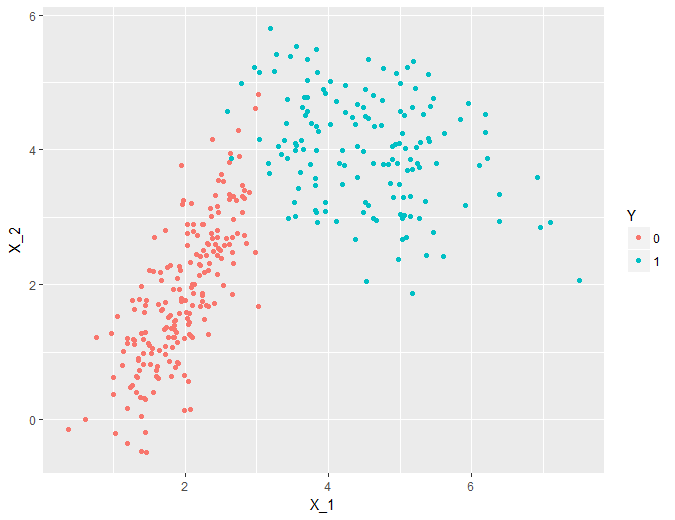
\includegraphics[width = .9\textwidth]{Tests/Test1/GroupPlot}
  \caption{Ejemplo 1, Poco traslape entre grupos}
 \label{fig:Test1Plot}
\end{figure}
Los parámetros se escogieron con un proceso de \textit{prueba y error} para dar estructura pero a la vez separación en el espacio de covariables $\mathcal{X}^2 \approx [0.3,7.5]\times[-0.5,5.9]$. Esto, para que se tuviera una pequeña región donde las distribuciones se traslaparan y exista cierto grado de confusión. El objetivo del modelo, es poder hacer una separación de estas dos regiones sin sobreajustar, identificando a grandes rasgos dónde se encuentran los puntos rojos y dónde se encuentran los puntos azules.

\subsubsection*{Modelo probit frecuentista para comparar}
En un modelo tradicional, la función de proyección lineal, rígida, y por ende la frontera de clasificación es lineal. Para comparar, se corrió el siguiente modelo probit frecuentista en \verb|R|, usando la función \verb|glm(..., family = binomial(link = 'probit'))|:
\begin{align}
	p_i & = P(y_i = 1) =\E[y|\xni] = \Phi(f(\xni))  \quad \Rightarrow  			\nonumber \\
	\Phi^{-1}(p_i) &= \beta_0 + \beta_1x_{i,1} + \beta_2x_{i,2} 
	\qquad 	\forall i =1,\ldots,n \label{ec:Test1ModGLM}
\end{align}
De donde se obtuvieron los resultados presentados en la tabla \ref{tab:Test0}

\begin{table}[h]
\begin{align*}
\begin{array}{c|c}
\text{Parámetro} &\text{Valor Estimado} \\
\hdashline
\hat{\beta_0} & -17.29 \\
\hat{\beta_1} & 4.43 \\
\hat{\beta_2} & 1.08 \\
\hline
\text{Métricas} & \text{Valor} \\
\hdashline
ll & 0.0399
\end{array}
\qquad\qquad\qquad
\matconf{198}{2}{200}{2}{148}{150}{200}{150}{350}
\end{align*}
\caption{Resultados para modelo probit}
\label{tab:Test0}
\end{table}

Dada la simplicidad de los datos, el modelo lineal probit, presentado en la ecuación (\ref{ec:Test1ModGLM}) resulta ser una excelente forma de hacer la clasificación. Como se ve en la Figura: \ref{fig:Test0ModGLM}, los datos son fácilmente separables por una linea recta que cruza exactamente donde se empiezan a traslapar. Únicamente, existen 4 datos que quedan mal clasificados, pero que, dadas sus coordenadas, parecerían pertenecer a los grupos opuestos y se consideran como datos atípicos. El modelo presenta una precisión de $98.85\%$, todos los parámetros fueron significativos\footnote{Usando las pruebas $t$ clásicas de modelos lineales frecuentistas.} y se tiene un valor de la función \textit{log-loss} muy bajo. Por lo tanto, se puede concluir que este modelo probit tradicional, es un muy buen modelo para este conjunto de datos. 
\begin{figure}[h]
  \centering
      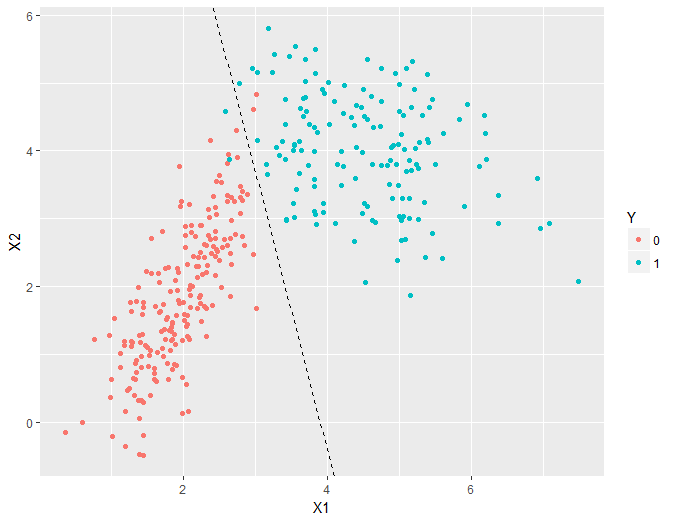
\includegraphics[width = .5\textwidth]{Tests/Test1/GLM_Line}
  \caption{Separación de los grupos por medio de un modelo probit lineal frecuentista}
 \label{fig:Test0ModGLM}
\end{figure}

\subsubsection*{Ejemplo 1: el modelo bpwpm} \label{sec:Test1Ej1}
Ahora, esta base de datos se prueba contra el modelo \textit{bpwpm} de este trabajo. Se esperaría que, al menos, se comportara como el probit anterior, pues, dada su estructura tan flexible, el modelo podría colapsar en uno lineal, replicando el probit tradicional anterior. 

Como un primer ejemplo sencillo de comprender, se corre un modelo donde los polinomios por partes son rectas disjuntas en cada segmento con un solo nodo. Se realizan mil simulaciones del muestreo Gibbs, de donde se descartan las primeras 500 observaciones y posteriormente se toma cada segunda observación. Estas especificaciones se resumen en la siguiente tabla que se presentará antes de cada modelo. 
\begin{table}[H]
$$\paramsmod{2}{2}{0}{4}{2}{350}{1000}{500}{2}$$
\caption{Ejemplo 1, rectas disjuntas, un solo nodo}
\label{ej:1}
\end{table}

Dado que este es un modelo extremadamente sencillo y que se tiene un número pequeño de bases para los polinomios por partes, $\N = 4$, se presenta por única ocasión, la expansión completa para poderla comparar contra el modelo anterior (\ref{ec:Test1ModGLM}). Esto es,\footnote{Para $w_{l,j}$, se usa la convención de subíndices $l = \for{1}{\N}$ de la biyección de la Tabla \ref{tab:Biyeccion} y $j = \for{1},{d}$ para indicar la dimensión}

\begin{align}
	p_i &= P(y_i = 1) =\E[y|\xni] = \Phi(f(\xni))  \quad \Rightarrow  			\nonumber \\
	\Phi^{-1}(p_i) = \;&\beta_0 + \beta_1f_1(x_{i,1}) + \beta_2f_2(x_{i,2}) 
	\qquad 	\forall i = \for{1,n}\label{ec:Test1Ej1} \\
	&= \beta_0 \nonumber \\
	&+ \beta_1[w_{1,1} + w_{2,1}x_{i,1} + w_{3,1} + w_{4,1}(x_{i,1} - \t_{1,1})_+] \label{ec:Test1Ej1F1}\\
	& +\beta_2[w_{1,2} + w_{2,2}x_{i,2} + w_{3,2} + w_{4,2}(x_{i,2} - \t_{1,2})_+]. \label{ec:Test1Ej1F2}
\end{align}

Contrastando la ecuación (\ref{ec:Test1ModGLM}) del modelo probit  contra (\ref{ec:Test1Ej1}) del modelo \textit{bpwpm}, se puede ver la introducción del componente no lineal a través de las funciones $f_j$ desglosadas en (\ref{ec:Test1Ej1F1}) y (\ref{ec:Test1Ej1F2}). El modelo , tiene un total de $1 + d + d\N = 11$ parámetros, recordando que los nodos son fijos. Las expansiones truncadas de polinomios son relativamente sencillas y se ve claramente que se les da estructura de recta, permitiendo discontinuidades entre ellas pues $(\cdot)_+$ es una función por partes que se activa si $x_{i,j}$ es mayor que el nodo $\tau{\cdot,j}$. Aunque esta expansión es aparatosa, el modelo logra hacer excelentes predicciones en cuanto a las regiones. Cabe mencionar que, dado este es un ejemplo introductorio con un número relativamente bajo de observaciones, la estimación de los parámetros, se realizó \textit{dentro de la muestra} (\textit{in-sample}) esto quiere decir, que el modelo se entrena con las mismas observaciones contra las que se busca predecir.\footnote{El efecto que esto podría tener es que se sobre-ajuste o se hagan predicciones demasiado acertadas, sin embargo, es normal hacerlo para este tipo de modelos dado $n$. Además, por lo pronto el objetivo final es dar predicciones a través de las regiones formadas y no tanto para observaciones nuevas. De cualquier forma, se podría hacer separando, antes del análisis, la base de datos en dos, una para entrenar el modelo y otra para probarlo.} 

Previo al análisis de convergencia de las cadenas, se hace una exploración preliminar para explicar todos los detalles del modelo. Usando la función de perdida cuadrática, se obtienen los resultados presentados en la Tabla \ref{tab:Test1Ej1Res}.

\begin{table}[h]
\begin{align*}
\resultados{\text{Media posterior}}{98.85}{0.03702}
\quad\quad
\begin{array}{c|c}
\multicolumn{2}{c}{\hat{\beta}} \\
\hline
\hat{\beta_0} & -0.79 \\
\hat{\beta_1} & 3.35 \\
\hat{\beta_2} & 0.65 \\
\end{array}
\quad\quad
\end{align*} 

\begin{align*}
\begin{array}{c|c}
\multicolumn{2}{c}{\hat{\wsn}} \\
\hline
-0.52 	& -1.48 \\
0.39	& -0.38 \\
0.09	& 0.66 \\
1.05	& 1.32
\end{array}
\quad\quad
\matconf{198}{2}{200}{2}{148}{150}{200}{150}{350}
\end{align*}
\caption{Ejemplo 1, resultados}
\label{tab:Test1Ej1Res}
\end{table}

Numéricamente, el modelo se ve bien; la matriz de confusión es idéntica a la del probit anterior y, por ende, la precisión. Sin embargo, se tiene un valor de la función \textit{log-loss} un poco más bajo, indicando que se tiene un mejor modelo una vez consideradas las probabilidades ajustadas $\hat{\psn}$. Sin embargo, a diferencia del modelo anterior, los parámetros estimados $\hat{\beta}$ y $\hat{\wsn}$ no se pueden interpretar de la misma manera. En modelos de ML, debido a la complejidad, es mejor tratar a los parámetros como partes funcionales del modelo, que como números con significado. Sin embargo en especial el vector $\hat{\beta}$ puede considerarse como los \textit{pesos} que se le dan a cada transformación no lineal, y su magnitud corresponde a que tanta fuerza tiene esa dimensión en el modelo. De este ejemplo se ve claramente que la primer dimensión, es con la que mejor se están explicando los datos.\footnote{Dado que se tiene una muestra arbitrariamente grande de los parámetros y se conoce su distribución, se podría probar la significancia de los parámetros.}

La Figura \ref{fig:Test1Ej1}, es clave para entender el modelo, en ella se presentan las dos regiones (de colores) que el modelo detecta para hacer las predicciones.

\begin{figure}[h]
	\centering
	\begin{subfigure}[b]{0.45\textwidth}
    	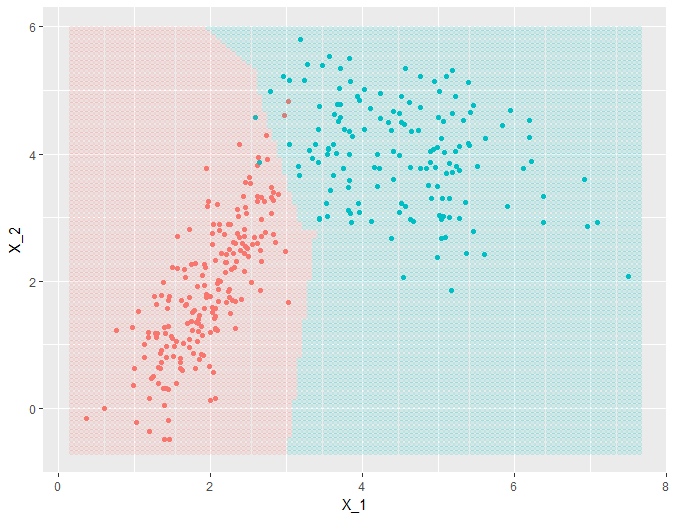
\includegraphics[width =\textwidth]{Tests/Test1/Ej1Frontera}
		\caption{Regiones de predicción para modelo con $M = 2$, $J = 2$ y $K = 0$}
	\label{fig:Test1Ej1}
	\end{subfigure}
	\hfill    
    \begin{subfigure}[b]{0.45\textwidth}
        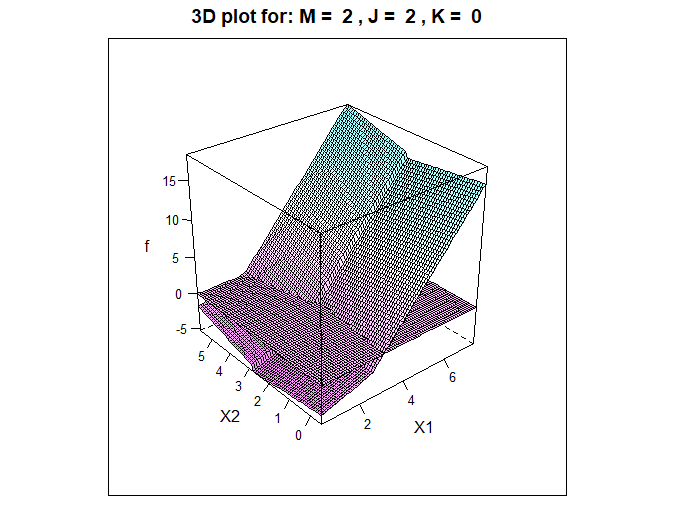
\includegraphics[width=\textwidth]{Tests/Test1/Ej13D}
        \caption{Representación en 3D de $\hat{f}$}
        \label{fig:Test1Ej13D}
    \end{subfigure}
    \caption{Ejemplo 1 con M = 2, J = 2, K = 0, modelo lineal discontinuo}
\end{figure}

A diferencia de los modelos lineales donde la frontera de predicción binaria es, por ende, lineal, el modelo presentado en este trabajo permite tener fronteras tan complejas como se quiera (aunque no siempre necesarias). Para este ejemplo en particular, la frontera refleja que se está usando un solo nodo y polinomios lineales discontinuos, es por ello que se da la rugosidad. Encontrar la frontera como tal, resulta una tarea mucho más complicada, pues correspondería a resolver la ecuación  $\hat{f}(\xsn) \equiv 0$; en los GLM, esta frontera es perfectamente lineal y el despeje se puede hacer. Sin embargo, cuando se tienen modelos no lineales, se puede hacer una proyección de ella pues, recordando, lo que interesa es discernir cuando la función $\hat{f}$ sea positiva o negativa. Gracias al hecho que $d = 2$ para este ejemplo, se puede visualizar $\hat{f}(\xsn)$ en la Figura \ref{fig:Test1Ej13D}. En esta gráfica, se marca con un plano el \textit{corte} cuando $\hat{f}(\xsn)$ se vuele positiva. Además. se detectan los \textit{pliegues} de discontinuidades derivados del nodo y de la especificación en los parámetros $\MJK$. Se hace notar, que esta representación, no es más que la suma ponderada (por $\hat{\beta})$ de las transformaciones no lineales $f_j \quad j=1,2$, por lo cual vale la pena visualizarlas en la Figura \ref{fig:Test1Ej1Fs}. 
\begin{figure}[h]
    \begin{subfigure}[b]{0.45\textwidth}
        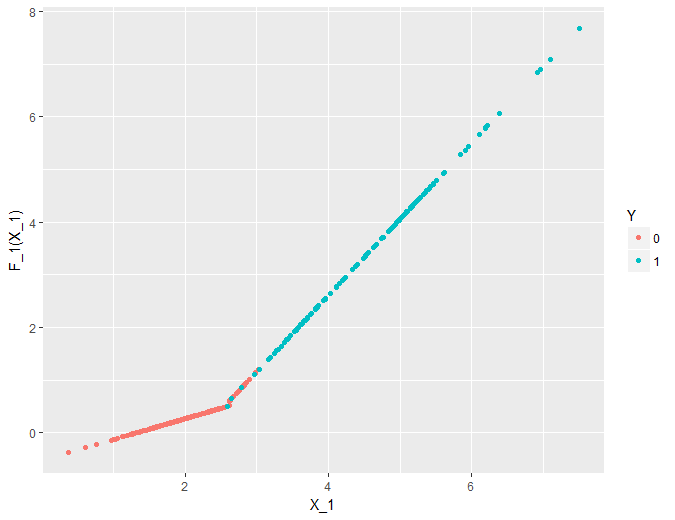
\includegraphics[width=\textwidth]{Tests/Test1/Ej1F1}
        \caption{$\hat{f}_1(x_1)$}
    \end{subfigure}
	\hfill
	    \begin{subfigure}[b]{0.45\textwidth}
        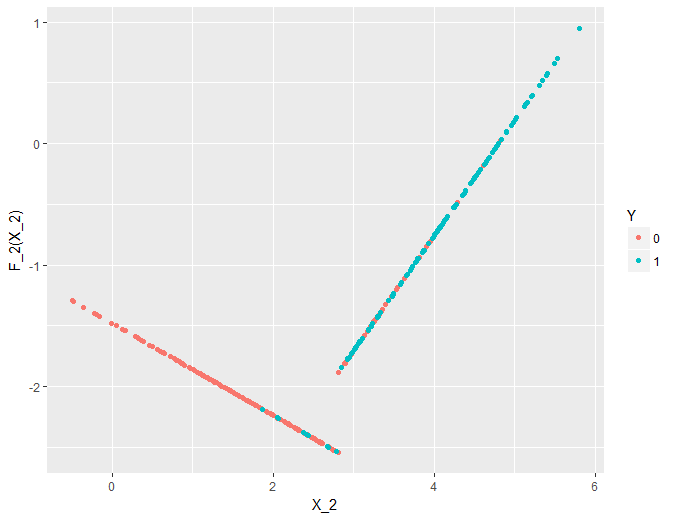
\includegraphics[width=\textwidth]{Tests/Test1/Ej1F2}
        \caption{$\hat{f}_2(x_2)$}
    \end{subfigure}
    \caption{Transformaciones no lineales para cada dimensión}\label{fig:Test1Ej1Fs}
\end{figure}
Aunque la escala vertical de $f_j$ es arbitraria, pues en realidad  están ajustando a los residuales parciales, las funciones están cumpliendo su propósito de detectar y capturar el patrón que deriva en la separación de los grupos. Para valores izquierdos de ambas variables, se tiene el grupo rojo, para valores mayores, se tiene el grupo azul. Ese efecto, es capturado en el salto que dan las rectas en el nodo, mediante una mayor pendiente en las rectas del lado derecho (mayoritariamente azules), pues, al ser más positivas conforme se avanza en el rango de $x$, estas tendrán más peso en la función de proyección $\hat{f}$, volviéndola más positiva y por ende, más probable que esa región contenga observaciones del grupo azul.

Con estas gráficas, se espera dar claridad a todos los componentes del modelo. Este ejemplo trivial, donde $d = 2$, tiene la ventaja que todo es visualizable gráficamente. Se hace énfasis en que muchas de las variables presentadas o métodos, son puramente estructurales y que cumplen una función meramente técnica en el algoritmo, como lo son las variables auxiliares $\zsn$. Al final, y como se presentó en el la Figura \ref{fig:DiagramaMod}, el modelo tiene cierta coherencia y simplicidad fácilmente representable por regiones de dos colores. Posteriormente, se verá la flexibilidad de estas regiones, ahí donde recae la fuerza del modelo.

Aunque las funciones $f_j$ sean relativamente sencillas presentadas en una dimensión como en la Figura \ref{fig:Test1Ej1Fs}, una vez colapsadas en la función de proyección $f$, se pueden tener efectos inesperados o relativamente extraños. Esto se debe a que la interacción entre los nodos en más de una dimensión puede ser complicada de visualizar y al juntar todo, se dan efectos como los pliegues de la figura \ref{fig:Test1Ej13D}. Para solucionar esto, usualmente se pide cierta suavidad en los polinomios por partes haciéndolos splines para que $f$ sea también suave. Sin embargo, dependiendo de la aplicación los parámetros $\MJK$ se van calibrando hasta que el modelo sea aceptable y las cadenas hayan convergido. 

\subsection{Diferentes tipos de fronteras - análisis de sensibilidad } \label{sec:AnlisisSensibilidad}
Toda la flexibilidad del modelo, depende de los parámetros $\MJK$ que recaen en las manos del estadista. Estos parámetros controlan la suavidad de la frontera y es importante que se entienda como cada uno afecta la estimación de los polinomios. Por lo tanto y para pasar de esta base de datos sencilla a algunas más retadoras, se juega un poco con ellos para ver sus efectos en el modelo. 

\subsubsection*{Ejemplo 2: polinomios constantes}
A principio, mientras se desarrollaba el paquete, parecía intuitivo
que, si se está construyendo una clasificación binaria, a cada observación bidimensional $\xni = (x_{i,1}, x_{i,2})^t$ se transformara en una especie de \textit{observación de diseño},\footnote{Derivado de las \textit{matrices de diseño} que se construyen para los modelos ANOVA; si se pudiera mapear cada observación a un espacio más sencillo codificando la respuesta, se podría hacer una predicción aún mejor.} la cual codificaría si su correspondiente respuesta $y_i$ era 0 o 1. Esta linea de pensamiento, llevo a pensar que escoger los polinomios por partes como constantes sería la mejor opción para la predicción y separación de las regiones. Por lo tanto, se corre el modelo con los parámetros presentados en la Tabla \ref{ej:2}.
\begin{table}[h]
$$\paramsmod{1}{2}{0}{2}{2}{350}{1000}{500}{2}$$
\caption{Ejemplo 2, rectas constantes, un solo nodo}
\label{ej:2}
\end{table}

De donde se obtiene los resultados presentados en la Tabla \ref{tab:Test1Ej2Res}. De ahora en adelante, y hasta llegar al análisis de convergencia, dado que la complejidad de los modelos comenzará a aumentar, se opta por no mostrar los estimadores $\hat{\beta}$ y $\hat{\wsn}$ pues no aportan nada a la discusión y son difícilmente interpretables. Se opta mejor por presentar las gráficas. 

\begin{table}[h]
\begin{align*}
\resultados{\text{Media posterior}}{92.3}{0.2081}
\qquad\qquad\qquad
\matconf{174}{26}{200}{1}{149}{150}{175}{175}{350}
\end{align*} 
\caption{Ejemplo 2, resultados}
\label{tab:Test1Ej2Res}
\end{table}

\begin{figure}[p]
        \centering
        \begin{subfigure}[b]{0.45\textwidth}
            \centering
            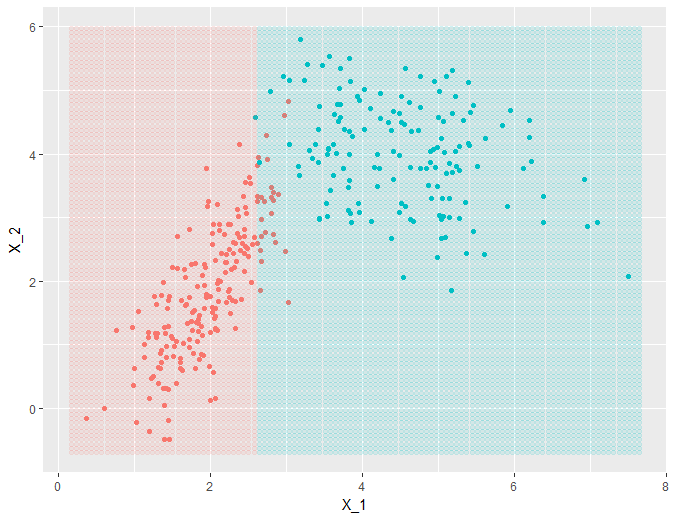
\includegraphics[width=\textwidth]{Tests/Test1/Ej2Frontera}
            \caption{Frontera}   
            \label{fig:Test1Ej2Frontera}
        \end{subfigure}
        \hfill
        \begin{subfigure}[b]{0.45\textwidth}  
            \centering 
            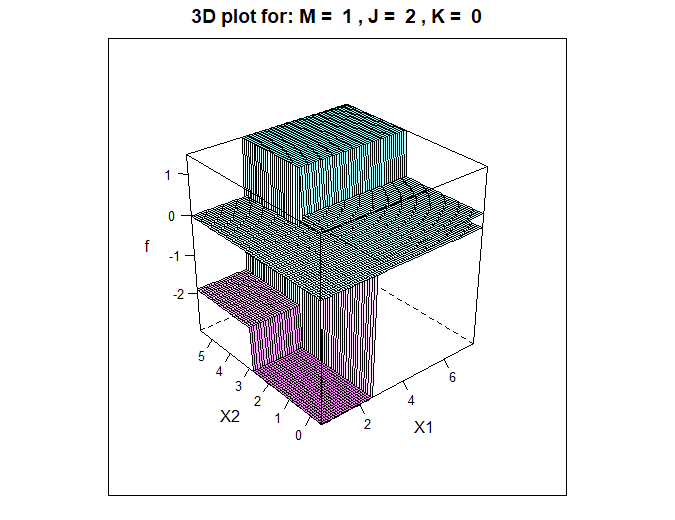
\includegraphics[width=\textwidth]{Tests/Test1/Ej23D}
            \caption{Representación 3D de $\hat{f}$}
            \label{fig:Test1Ej23D}
        \end{subfigure}
        \vskip\baselineskip
        \begin{subfigure}[b]{0.45\textwidth}   
            \centering 
            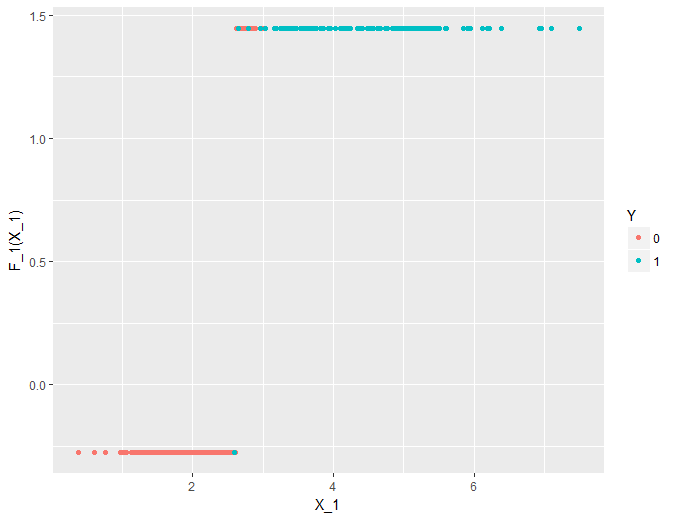
\includegraphics[width=\textwidth]{Tests/Test1/Ej2F1}
            \caption{$\hat{f}_1(x_1)$}
            \label{fig:Test1Ej2F1}
        \end{subfigure}
        \quad
        \begin{subfigure}[b]{0.45\textwidth}   
            \centering 
            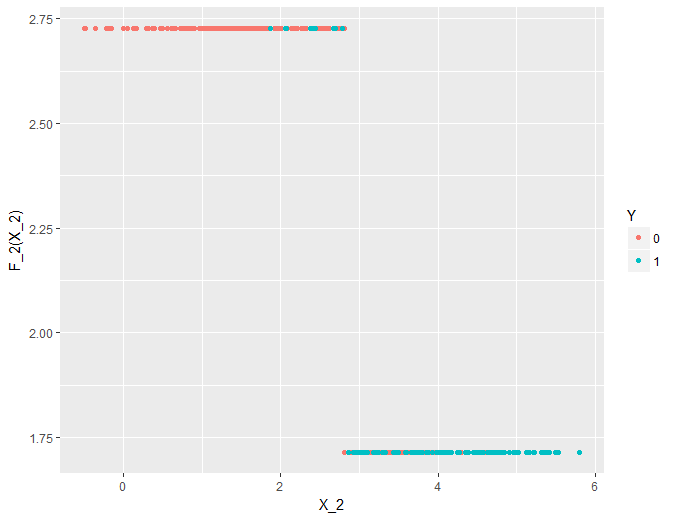
\includegraphics[width=\textwidth]{Tests/Test1/Ej2F2}
            \caption{$\hat{f}_2(x_2)$}    
            \label{fig:Test1Ej2F2}
        \end{subfigure}
        \caption{Ejemplo 2 con $M = 1$, $J = 2$, $K = 0$, función escalonada}
        \label{fig:Test1Ej2Plots}
\end{figure}
Claramente, esta no es una mejora al modelo. Tanto en precisión como en métrica \textit{log-loss} el modelo empeoró significativamente. En la Figura\ref{fig:Test1Ej2Plots}, se visualiza el porqué. Al tener únicamente un nodo y polinomios por partes constantes, la región de predicción es la más sencilla posible: dos planos que separan las regiones rojas y azules. En la imagen \ref{fig:Test1Ej23D}, se visualiza la función escalonada resultante con 4 \textit{mesetas} producto de las interacciones entre los dos nodos. Se hace notar que la región inferior izquierda es más negativa pues se tiene menor probabilidad de ser del grupo azul. En las imágenes \ref{fig:Test1Ej2F1} y \ref{fig:Test1Ej2F2} se ven los polinomios constantes que siguen el diseño del experimento, esto es, codificar de forma más sencilla la variable real $\xsn$, sin embargo, al considerar las interacciones entre los nodos, la intuición se pierde. Se hace notar que en la Figura \ref{fig:Test1Ej2F2} los polinomios están invertidos, esto se debe a que $\beta_2$ se estimó negativo, por lo tanto, a mayores valores de $\hat{f_2}$, la $f$ global aumenta, indicando que los parámetros están captando bien los patrones.

\subsubsection*{Ejemplo 3: aumento del número de nodos}

Como un tercer ejemplo, se podría pensar que aumentando el número de nodos y dejando todo lo demás constante mejoraría la predicción, sin embargo, lo hace de forma marginal. Tomando $J = 3$ (equivalente a dos nodos) se obtiene una precisión del $95.7\%$, en la Figura \ref{fig:Test1Ej3Plots} se presentan los resultados visuales. Se hace notar, que en este caso en especifico, si la posición del segundo nodo en $x_1$ fuera ligeramente menor ($x_1 \approx 3$) la región de predicción mejoraría. De igual forma, se hace notar que se tienen $J^2 = 9$ mesetas en la representación 3D y que, en las regiones de confusión, las $f_j$ tienen valores más cercanos a cero, identificando esta incertidumbre.

\begin{figure}[p]
        \centering
        \begin{subfigure}[b]{0.45\textwidth}
            \centering
            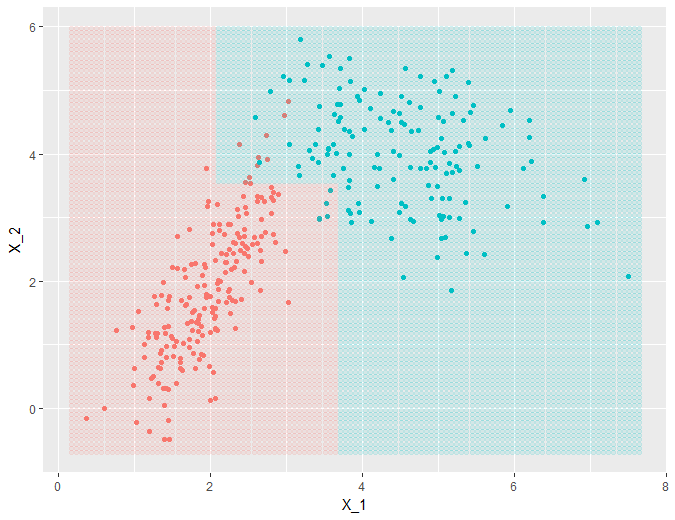
\includegraphics[width=\textwidth]{Tests/Test1/Ej3Frontera}
            \caption{Frontera}   
            \label{fig:Test1Ej3Frontera}
        \end{subfigure}
        \hfill
        \begin{subfigure}[b]{0.45\textwidth}  
            \centering 
            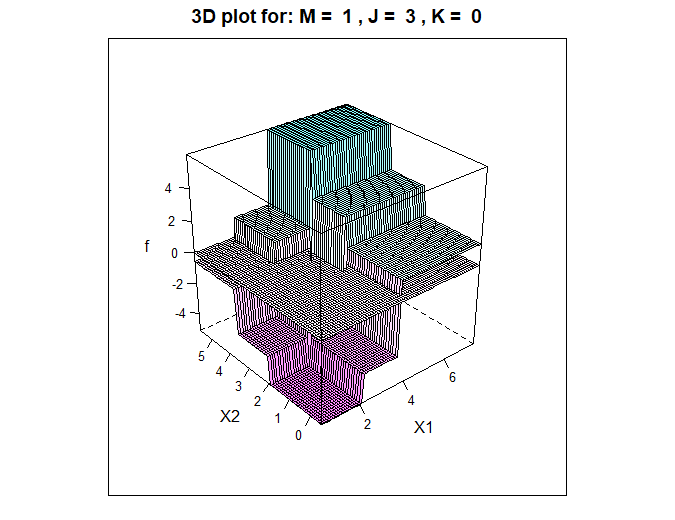
\includegraphics[width=\textwidth]{Tests/Test1/Ej33D}
            \caption{Representación 3D de $\hat{f}$}
            \label{fig:Test1Ej33D}
        \end{subfigure}
        \vskip\baselineskip
        \begin{subfigure}[b]{0.45\textwidth}   
            \centering 
            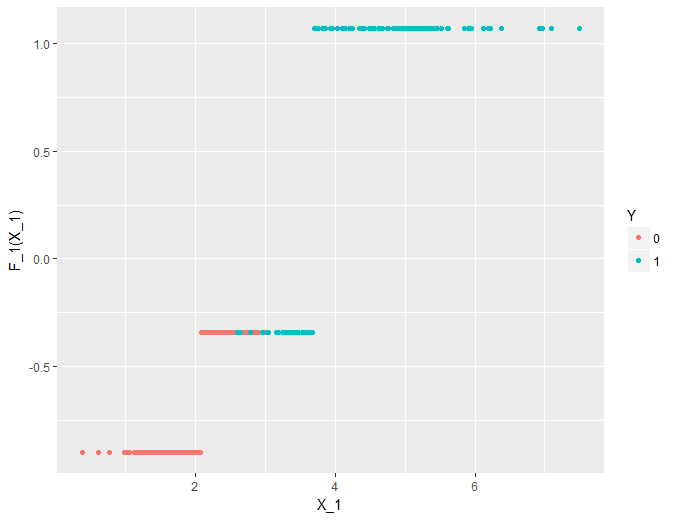
\includegraphics[width=\textwidth]{Tests/Test1/Ej3F1}
            \caption{$\hat{f}_1(x_1)$}
            \label{fig:Test1Ej3F1}
        \end{subfigure}
        \quad
        \begin{subfigure}[b]{0.45\textwidth}   
            \centering 
            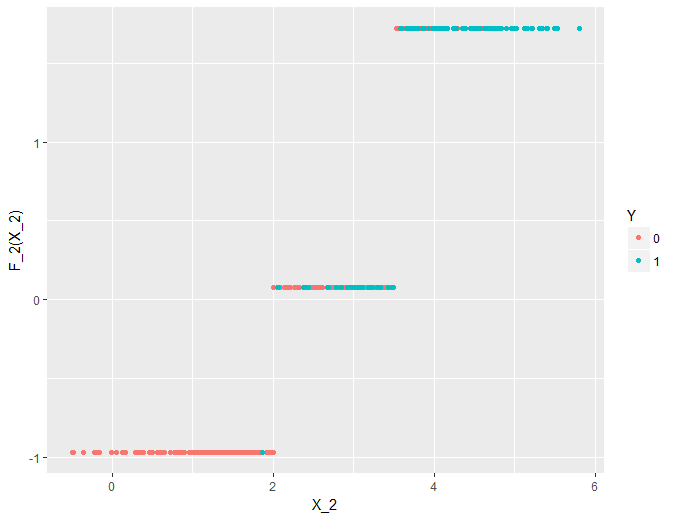
\includegraphics[width=\textwidth]{Tests/Test1/Ej3F2}
            \caption{$\hat{f}_2(x_2)$}    
            \label{fig:Test1Ej3F2}
        \end{subfigure}
        \caption{Ejemplo 3 con $M = 1$, $J = 3$, $K = 0$}
        \label{fig:Test1Ej3Plots}
\end{figure}
Seguir aumentando el número de nodos, no mejora sustancialmente la estimación. Por lo tanto, lo que se debe hacer es romper la linealidad aumentando $M$ y $K$.

\subsubsection*{Ejemplo 4: linealidad + continuidad}
Para el primer ejemplo de la Sección \ref{sec:Test1Ej1}, se usaron los parámetros, $M = 2$, $J = 2$ y $K = 0$. Esto corresponde a expansiones polinómicas lineales pero discontinuas. Parecería contra-intuitivo usar polinomios continuos en los nodos pensando en que se buscan predicciones binarias, sin embargo, resulta que al aumentar la \textit{suavidad} en los polinomios, se logra al menos igualar el nivel de precisión para este ejemplo. En otras bases de datos se verá que esta suavidad es inclusive necesaria para dar mejores predicciones. Asimismo, se ve empiricamente, que al aumentar el numero de parámetros y la suavidad, se tienen estimaciones más robustas que convergen mejor a distribuciones estacionarias. Esto se debe a que al aumentar el número de variables (en este caso dos) las fronteras flexibles, logran aproximar de mejor manera la frontera real. 

Para este nuevo ejemplo, se aumenta $K = 1$ haciendo que la doble suma en la expansión de bases de \ref{ec:PoliMallik} de la página \ref{ec:PoliMallik} se desvanezca regresando a la definición de splines lineales. Se tiene el modelo resumido en la Tabla \ref{ej:4}, con sus correspondientes resultados presentados en la Tabla \ref{tab:Test1Ej4Res}. 

\begin{table}[h]
$$\paramsmod{2}{2}{1}{3}{2}{350}{1000}{500}{2}$$
\caption{Ejemplo 4, rectas continuas, un nodo}
\label{ej:4}
\end{table}

\begin{table}[h]
\begin{align*}
\resultados{\text{Media posterior}}{98.85}{0.04109}
\qquad\qquad\qquad
\matconf{198}{2}{200}{2}{148}{150}{200}{150}{350}
\end{align*}
\caption{Ejemplo 4, resultados}
\label{tab:Test1Ej4Res}
\end{table}

Este modelo es igual de bueno que el primer ejemplo, pero con un valor de \textit{log-loss} marginalmente mayor. Una vez más, se presentan las cuatro imágenes habituales para evaluarlo en la Figura \ref{fig:Test1Ej4Plots}. Otra característica contra-intuitiva de este modelo en particular, es que se tiene un parámetro menos para cada expansión de bases, ahora $\N = 3$, pues al añadir la restricción de continuidad por nodo se elimina uno de los dos términos independientes en las expansiones de las ecuaciones (\ref{ec:Test1Ej1F1}) y (\ref{ec:Test1Ej1F2}).  
\begin{figure}[p]
        \centering
        \begin{subfigure}[b]{0.45\textwidth}
            \centering
            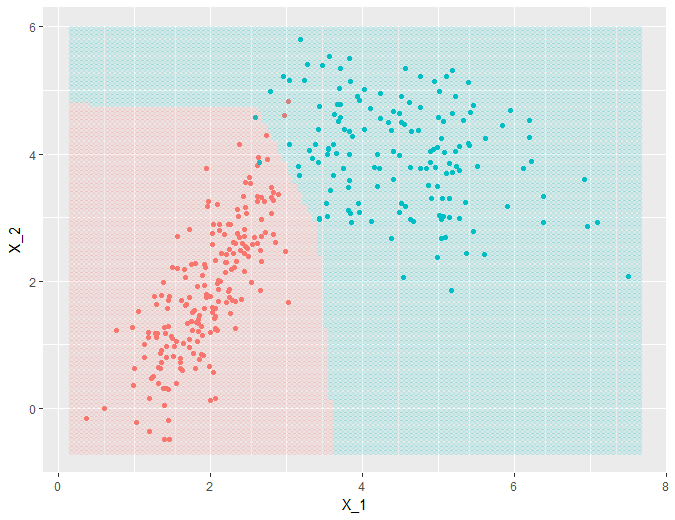
\includegraphics[width=\textwidth]{Tests/Test1/Ej4Frontera}
            \caption{Frontera}   
            \label{fig:Test1Ej4Frontera}
        \end{subfigure}
        \hfill
        \begin{subfigure}[b]{0.45\textwidth}  
            \centering 
            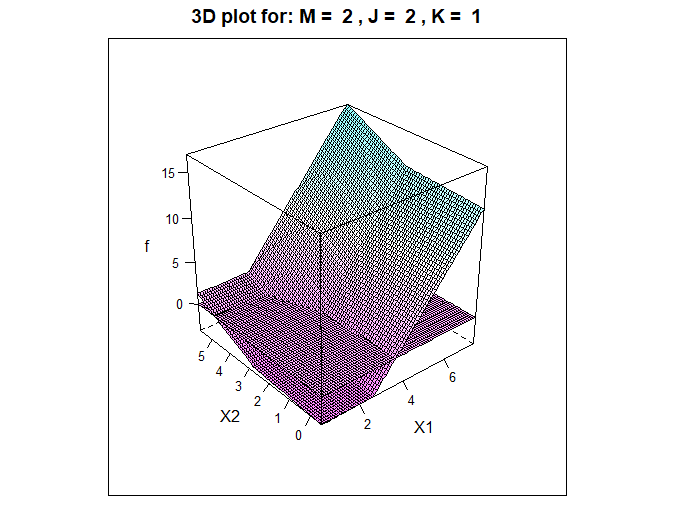
\includegraphics[width=\textwidth]{Tests/Test1/Ej43D}
            \caption{Representación 3D de $\hat{f}$}
            \label{fig:Test1Ej43D}
        \end{subfigure}
        \vskip\baselineskip
        \begin{subfigure}[b]{0.45\textwidth}   
            \centering 
            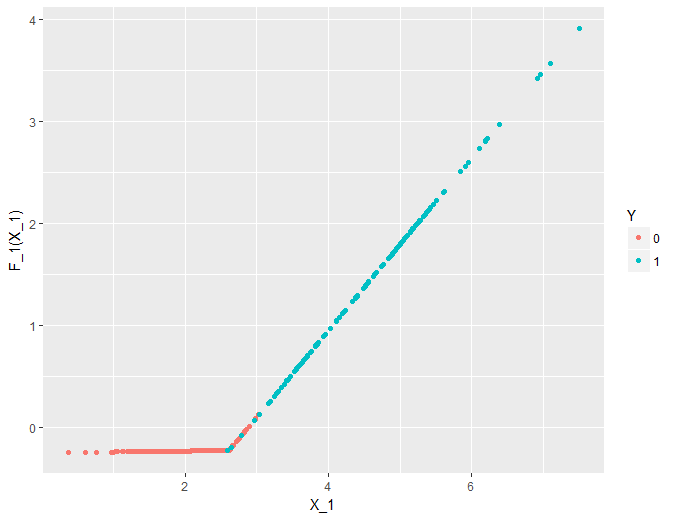
\includegraphics[width=\textwidth]{Tests/Test1/Ej4F1}
            \caption{$\hat{f}_1(x_1)$}
            \label{fig:Test1Ej4F1}
        \end{subfigure}
        \quad
        \begin{subfigure}[b]{0.45\textwidth}   
            \centering 
            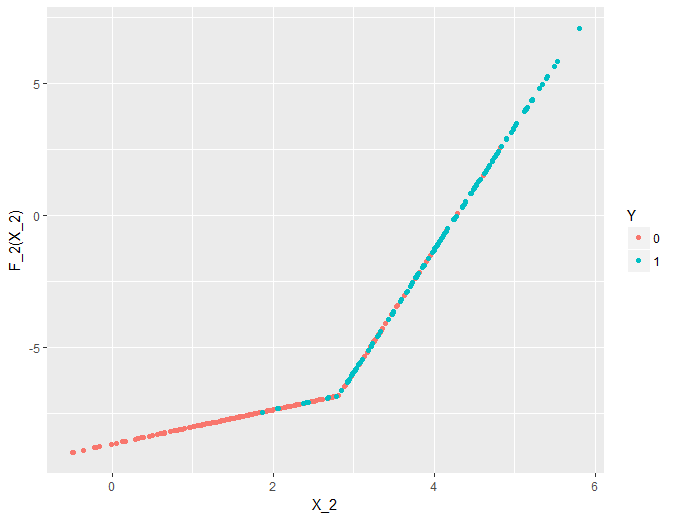
\includegraphics[width=\textwidth]{Tests/Test1/Ej4F2}
            \caption{$\hat{f}_2(x_2)$}    
            \label{fig:Test1Ej4F2}
        \end{subfigure}
        \caption{Ejemplo 4 con $M = 2$, $J = 2$, $K = 1$, modelo lineal continuo}
        \label{fig:Test1Ej4Plots}
\end{figure}
Con estas imágenes, es claro ver que se está buscando mayor suavidad progresivamente. En \ref{fig:Test1Ej43D}, se ve que la \textit{sabana} ya no da brincos discontinuos y, aunque aún no sea suave, si retiene la estructura de predicción. Esta frontera se aprecia mejor en \ref{fig:Test1Ej4Frontera}, donde se ve claramente como el modelo logra detectar perfectamente bien la región problemática. Finalmente, de \ref{fig:Test1Ej4F1} y \ref{fig:Test1Ej4F2}, se pueden apreciar las rectas ya continuas. Analizándolas, se ve claramente que existe muy poca confusión en cuanto a la primera región roja por lo que $\hat{f}_1(x_1)$ es plana al principio y después comienza a crecer rápidamente. Sucede lo mismo con $\hat{f}_2(x_2)$, sin embargo, la escala es un poco diferente, ya que $\hat{\beta}_2$ es cercana a cero, confirmando la creencia de que la región se puede separar de manera excelente, únicamente con la información de $x_1$.\footnote{Aunque no se implementaron, técnicas de \textit{selección de variables} también podrían ser útiles.} Asimismo, aumentar el número de nodos ya no mejora significativamente el modelo y sólo le agrega más parámetros por estimar. 

\subsubsection*{Ejemplo 5 y 6: polinomios de orden mayor} \label{sec:Test1Ej6}
Para cerrar las pruebas con esta base de datos y empezar a probarlo en regiones más interesantes, se corren dos últimos modelos con polinomios de orden mayor. En particular para el ejemplo 5, se usan parábolas discontinuas con 2 nodos para ver las capacidades del modelo. Finalmente para el ejemplo 6 se usan los famosos splines cúbicos para ver que tan suave puede llegar a ser el modelo. 
\begin{table}
	\begin{subtable}{0.45\textwidth}
	\centering
	$\paramsmod{3}{3}{0}{9}{2}{350}{1000}{500}{2}$
	\caption{Ejemplo 5, parábolas discontinuas}
	\label{ej:5}
	\end{subtable}
	\quad
	\begin{subtable}{0.45\textwidth}
	\centering
	$\paramsmod{4}{3}{3}{6}{2}{350}{2000}{1000}{3}$	
	\caption{Ejemplo 6, splines cúbicos}
	\label{ej:6}
	\end{subtable}
\end{table}

Se hace notar, que para el ejemplo 6 se corre una cadena relativamente más larga y con periodo de \textit{burn-in} $k^*$ también mayor. Esto se debe a el ejemplo 6 es el elegido para analizar su convergencia en la Sección \ref{sec:AnalisisConv} pues se dan resultados interesantes.

Para el ejemplo 5, se obtuvieron los resultados presentados en la Tabla \ref{tab:Test1Ej5Res} con sus respectivas imágenes presentadas en la Figura \ref{fig:Test1Ej5Plots}.
\begin{table}[h]
\begin{align*}
\resultados{\text{Media posterior}}{98.85}{0.03189}
\qquad\qquad\qquad
\matconf{198}{2}{200}{2}{148}{150}{200}{150}{350}
\end{align*}
\caption{Ejemplo 5, resultados}
\label{tab:Test1Ej5Res}
\end{table}

\begin{figure}[p]
        \centering
        \begin{subfigure}[b]{0.45\textwidth}
            \centering
            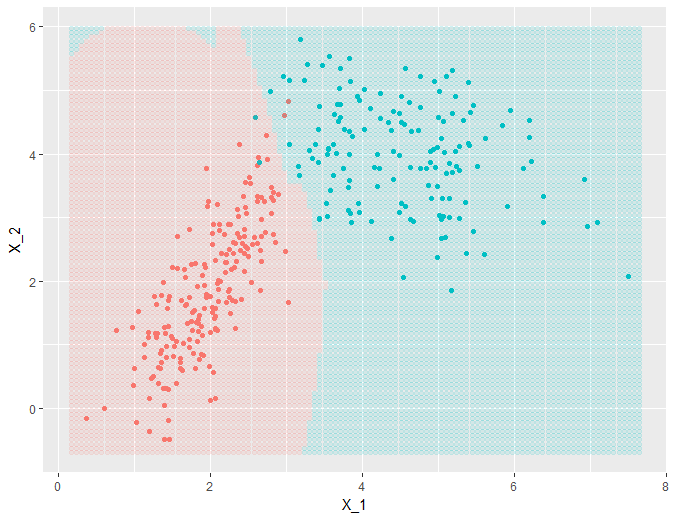
\includegraphics[width=\textwidth]{Tests/Test1/Ej5Frontera}
            \caption{Frontera}   
            \label{fig:Test1Ej5Frontera}
        \end{subfigure}
        \hfill
        \begin{subfigure}[b]{0.45\textwidth}  
            \centering 
            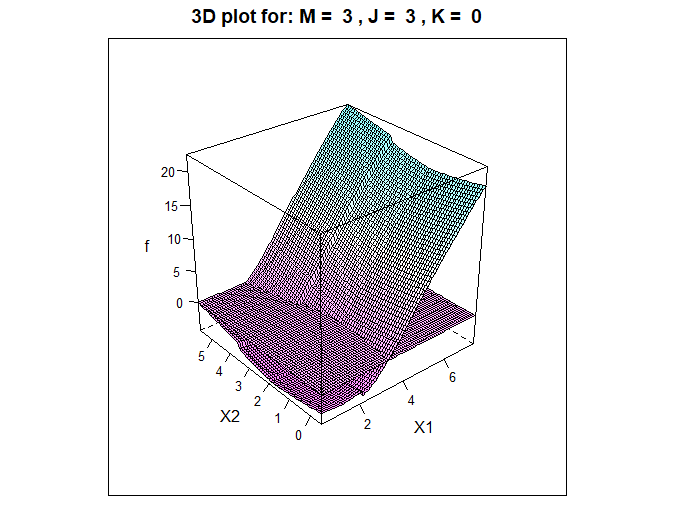
\includegraphics[width=\textwidth]{Tests/Test1/Ej53D}
            \caption{Representación 3D de $\hat{f}$}
            \label{fig:Test1Ej53D}
        \end{subfigure}
        \vskip\baselineskip
        \begin{subfigure}[b]{0.45\textwidth}   
            \centering 
            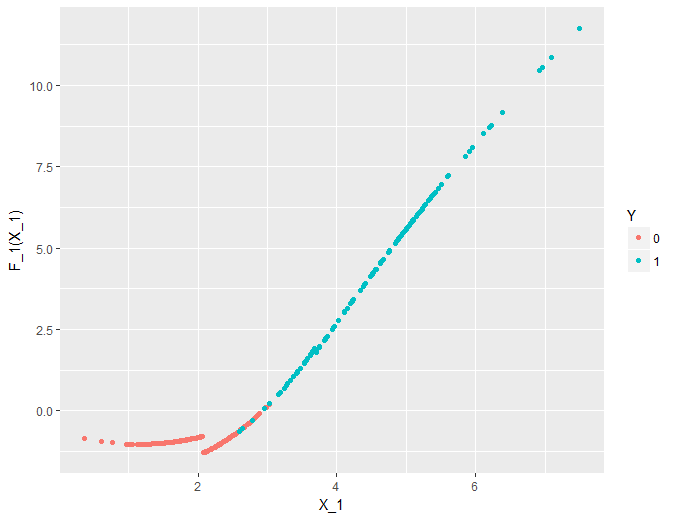
\includegraphics[width=\textwidth]{Tests/Test1/Ej5F1}
            \caption{$\hat{f}_1(x_1)$}
            \label{fig:Test1Ej5F1}
        \end{subfigure}
        \quad
        \begin{subfigure}[b]{0.45\textwidth}   
            \centering 
            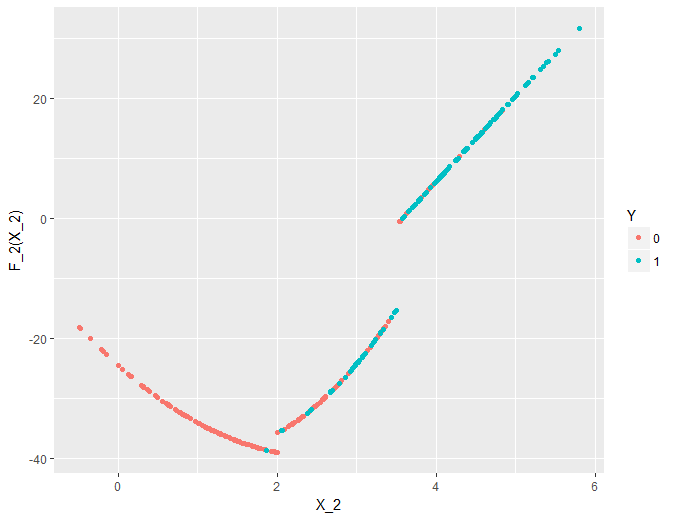
\includegraphics[width=\textwidth]{Tests/Test1/Ej5F2}
            \caption{$\hat{f}_2(x_2)$}    
            \label{fig:Test1Ej5F2}
        \end{subfigure}
        \caption{Ejemplo 5 con $M = 3$, $J = 3$, $K = 0$, parábolas discontinuas}
        \label{fig:Test1Ej5Plots}
\end{figure}
De donde lo único diferente es la forma de las funciones $\hat{f}_j$. La Figura \ref{fig:Test1Ej5F1}, presenta un comportamiento interesante: se conserva algo de la continuidad, casi como si las parábolas \textit{quisieran} ser continuas pues esa es la mejor opción para la predicción. Asimismo \ref{fig:Test1Ej53D} y \ref{fig:Test1Ej5Frontera} presentan claramente los efectos de las discontinuidades derivados de elegir $K = 0$. Este ejemplo, funciona mejor como un referente de las capacidades del modelo preservando la precisión, en la práctica tener 21 parámetros para un ejemplo tan sencillo no es nada útil.

Finalmente, el ejemplo 6, es más de lo mismo, los resultados son prácticamente iguales que los obtenidos con los demás modelos. 
%Esta similitud, se debe al hecho que la base de datos es muy sencilla.
Sin embargo, se presentan las imágenes en la Figura \ref{fig:Test1Ej6Plots} donde se puede ver claramente la \textit{suavidad} obtenida en la frontera, en la función $\hat{f}$ y las correspondientes $\hat{f}_j$. 
\begin{figure}[p]
        \centering
        \begin{subfigure}[b]{0.45\textwidth}
            \centering
            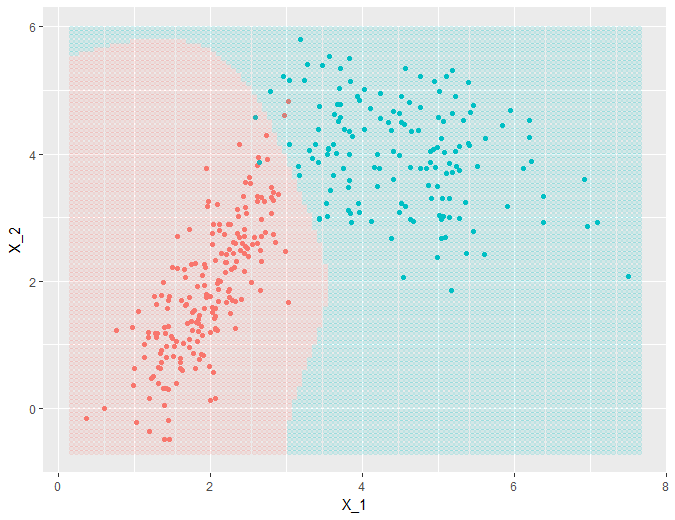
\includegraphics[width=\textwidth]{Tests/Test1/Ej6Frontera}
            \caption{Frontera}   
            \label{fig:Test1Ej6Frontera}
        \end{subfigure}
        \hfill
        \begin{subfigure}[b]{0.45\textwidth}  
            \centering 
            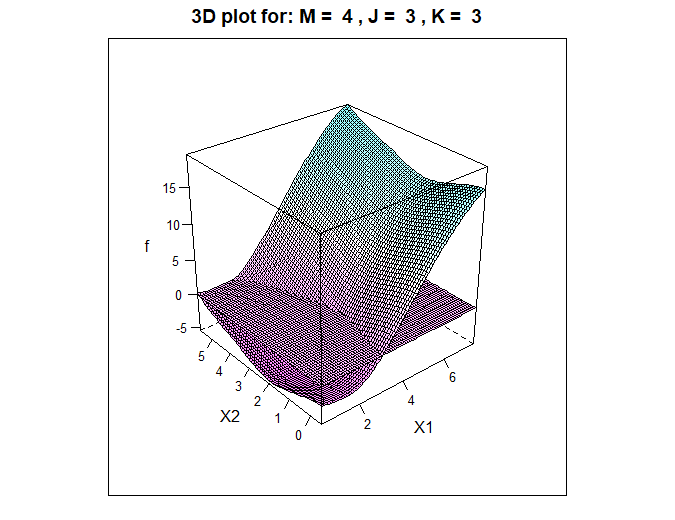
\includegraphics[width=\textwidth]{Tests/Test1/Ej63D}
            \caption{Representación 3D de $\hat{f}$}
            \label{fig:Test1Ej63D}
        \end{subfigure}
        \vskip\baselineskip
        \begin{subfigure}[b]{0.45\textwidth}   
            \centering 
            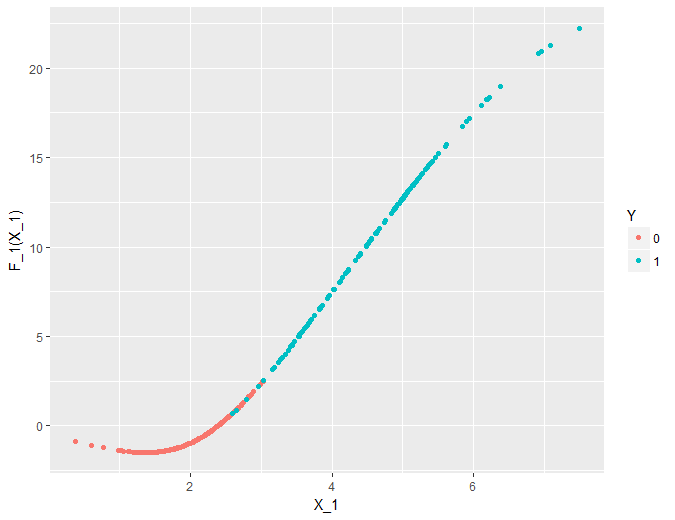
\includegraphics[width=\textwidth]{Tests/Test1/Ej6F1}
            \caption{$\hat{f}_1(x_1)$}
            \label{fig:Test1Ej6F1}
        \end{subfigure}
        \quad
        \begin{subfigure}[b]{0.45\textwidth}   
            \centering 
            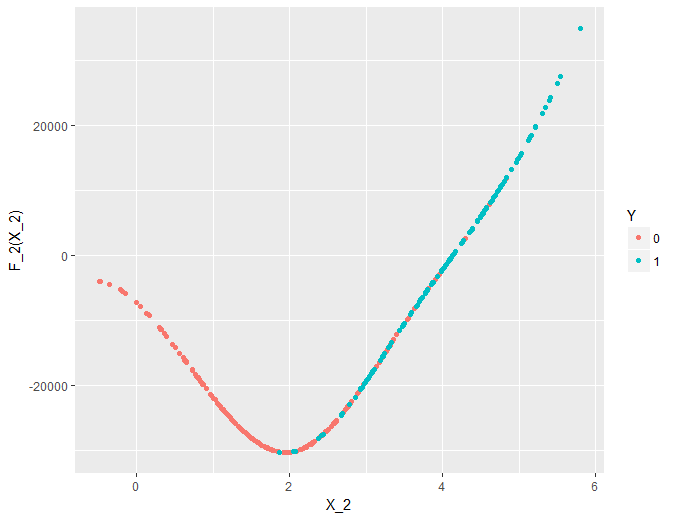
\includegraphics[width=\textwidth]{Tests/Test1/Ej6F2}
            \caption{$\hat{f}_2(x_2)$}    
            \label{fig:Test1Ej6F2}
        \end{subfigure}
        \caption{Ejemplo 6 con $M = 4$, $J = 3$, $K = 3$, splines cúbicos}
        \label{fig:Test1Ej6Plots}
\end{figure}
Al tener una cadena más larga, la escala de las $\hat{f}_j$, empieza a ser relativamente arbitraria, sobre todo para la segunda pues, conforme converge el modelo los parámetros $\wsn$ compensan la escala de $\beta$ y viceversa. Se continúa con este ejemplo en la siguiente sección.

En la practica, escoger el \textit{mejor} modelo es subjetivo pues depende del proceso de calibración de los parámetros y los resultados que se busquen obtener. Dado que el algoritmo es rápido, sobre todo para $d$ pequeñas, se puede jugar mucho con el, y explorar una serie de modelos. En casi todos los ejemplos presentados en esta base de datos se obtuvo una precisión de $98.85\%$, sería inverosímil tratar de mejorarla pues obligaría al modelo a sobreajustar y hacer regiones pequeñas para los 4 puntos que quedan en regiones de predicción opuestas. Asimismo, el número de nodos, al menos en este ejemplo, parece no importar mucho, aumentarlo, únicamente aumenta la complejidad del modelo y no aporta mucho, se ve claramente que con pocos parámetros y nodos, se tiene excelentes resultados. 

Como comentario final, se hace notar que dado el algoritmo es \textit{estocástico} y depende de la simulación de parámetros aleatorios, replicar exactamente las cadenas es una tarea casi imposible; mas, los resultados y las regiones son consistentes. Al menos para este ejemplo, los valores de $k^*$ y $\kthin$ también parecieran no importar mucho pues las cadenas convergen muy rápido por las propiedades de las distribuciones conjugadas usadas. 

\subsection{Análisis de convergencias} \label{sec:AnalisisConv}
El ejemplo 6 es interesante, pues ya se había explorado, sin saberlo, cuando se hablo de mustreo Gibbs en la sección \ref{sec:GibbsSampler}. En la Figura \ref{fig:GibbsSamplerSimulado} de la página \pageref{fig:GibbsSamplerSimulado}, se aprecian las trazas y los histogramas de los parámetros $\beta$ derivados de la simulación del modelo. Analizando la imagen \ref{fig:GibbsChain}, a primera vista, se observan varias cosas; la linea azul, que representa el parámetro $\hat{\beta}_2$ es prácticamente cero, la linea verde del parámetro $\hat{\beta}_1$ es muy consistente, casi sin variar, y la traza de $\hat{\beta}_0$ sube y baja sin aparente patrón. La imagen \ref{fig:GibbsChain} únicamente confirma esta creencia.

Este es el inicio de un análisis de convergencia más profundo que se debe realizar independientemente de los resultados tan positivos que se mostraron anteriormente. Pues, se recuerda, que estos fueron derivados de estimaciones puntuales para los parámetros usando la media posterior, la cual, no se sabe si es exacta o si depende de la sección que se tome de la cadena. Asimismo, este proceso se debe realizar para todos los parámetros del modelo, es decir, además de $\beta$, se deben estudiar los vectores $w_j \quad j = 1,2$. Por lo tanto, se realiza un análisis exploratorio de estas cadenas usando tres fuentes de información. Primero, se presentan resúmenes numéricos en la Tabla \ref{tab:ParametrosConv} para todos los parámetros del modelo una vez \textit{corregidas} las cadenas.\footnote{Descartando las observaciones antes de $k^*$ y adelgazando cada $\kthin$-ésimo valor} Después se contrastan estos números con la Figura \ref{fig:ACGibbs}, donde se  analizan gráficamente las cadenas por si mismas. Por último, en la Figura \ref{fig:ACEM}, se presentan las \textit{medias ergódicas} de las cadenas. Esta medida, no es más que la media acumulada de la cadena, la cual, se espera coincidan de forma muy puntual al valor de la media posterior. Con toda esta información, se puede formar una pintura completa de la estimación y convergencia de los parámetros del modelo.

\begin{table}[p]
	\centering
	\begin{subtable}{\textwidth}
		$\arraycolsep=12pt
		\begin{array}{l|c:c:c}
		\text{Métrica} &	\hat{\beta}_0 & \hat{\beta}_1 & \hat{\beta}_2\\
		\hline
		\text{Mínimo}              & -3.34 & 0.63 & 0.00 \\
		\text{Primer Cuartíl}      & -2.50 & 0.79 & 0.00 \\
		\text{Media}               & -1.65 & 0.82 & 0.00 \\
		\text{Mediana}             & -1.74 & 0.81 & 0.00 \\
		\text{Tercer Cuartíl}      & -0.93 & 0.85 & 0.00 \\
		\text{Máximo}              & 1.01 & 0.99 & 0.00 \\
		\text{Desviación Estandar} & 0.93 & 0.06 & 0.00 \\
		\end{array}$
	%\caption{\hat{\beta}}
	\end{subtable}
	\vskip\baselineskip
	\begin{subtable}{\textwidth}
		$\begin{array}{l|c:c:c:c:c:c}
		\multicolumn{7}{c}{\hat{w}_1} \\
		\text{Métrica} & \hat{w}_{1,1} & \hat{w}_{1,2} & \hat{w}_{1,3} & \hat{w}_{1,4} & \hat{w}_{1,5} & \hat{w}_{1,6} \\
        \hline                    
        \text{Mínimo} 			& -12.60 & -9.18 & -23.62 & -0.14 & -16.06 & -1.59 \\
        \text{Primer Cuartíl} 	& -2.44  & -2.87 & -2.27  & 0.45  & -3.31  & 0.28  \\
        \text{Media} 			& -1.55  & -1.94 & -1.64  & 0.97  & -2.27  & 1.46  \\
        \text{Mediana} 			& -1.24  & -1.56 & -1.20  & 0.69  & -1.53  & 0.88  \\
        \text{Tercer Cuartíl} 	& -0.32  & -0.72 & -0.53  & 1.30  & -0.90  & 2.29  \\
        \text{Máximo} 			& 15.22  & 4.67  & 4.10   & 7.74  & 0.60   & 11.55 \\
        \text{Desviación Estandar} & 2.10   & 1.74  & 1.94   & 0.78  & 1.98   & 1.84 
		\end{array}$
	%\caption{$\hat{w}_1$}
	\end{subtable}	
	\vskip\baselineskip
	\begin{subtable}{\textwidth}	
		$\begin{array}{l|c:c:c:c:c:c}
		\multicolumn{7}{c}{\hat{w}_2} \\
		\text{Métrica} & \hat{w}_{2,1} & \hat{w}_{2,2} & \hat{w}_{2,3} & \hat{w}_{2,4} & \hat{w}_{2,5} & \hat{w}_{2,6} \\
        \hline                    
		\text{Mínimo} 			& 0.00 & -61080 &  -46710	&  -7448 &	-25550  &  0.00 \\
		\text{Primer Cuartíl} 	& 0.00 &  -7509 &  -5396	&  77.7	 &	-4444   &  -43.9 \\
		\text{Media} 			& 0.00 &  -4693 &  -3515	&  1543  &	-2917   &  160.07 \\
		\text{Mediana} 			& 0.00 &  -2846 &  -1887	&  1227  &	-2320   &  355.6 \\
		\text{Tercer Cuartíl} 	& 0.00 &    -69 &    -82	&  2293  &	-103.2  &  3185 \\
		\text{Máximo} 			& 0.00 &  29420 &  36720	&  4110  &	14410   &  3092 \\
		\text{Desviación Estandar} & 0.00 &   7147 &   5691	&  1799  &	3562    &  452 
		\end{array}$
	%\caption{$\hat{w}_2$}
	\end{subtable}
	\caption{Resúmenes numéricos para los parámetros del modelo presentado en el ejemplo 6}
	\label{tab:ParametrosConv}
\end{table}

Para los parámetros $\hat{\beta}$, las medias y las medianas son en general similares como se aprecia en la imágenes \ref{fig:ACBetaChain} y \ref{fig:ACBetaHist}. Por un lado, $\hat{\beta}_0$ fluctúa bastante, teniendo un rango máximo de 4 unidades y una desviación estándar de casi una unidad, sin embargo, el rango intercuartílico queda consistentemente en los números negativos. Análizando sus medias ergódicas, tanto la total en  \ref{fig:ACEMBetaToda} como la parcial \ref{fig:ACEMBetaParcial}, se confirma que $\hat{\beta}_0$ está convergiendo a valores negativos alrededor de $-1$. Aunque su valor fluctúa y no es el más consistente, lo importante es que sea negativo y su media es un valor que funciona en la práctica. Por el otro lado, $\hat{\beta}_1$ tiene resultados más precisos confirmado por todas sus gráficas. La traza casi no varia, y tomando la segunda mitad de la cadena, su valor converge a algo cercano de $0.8$. La estabilidad de $\hat{\beta}_1$, se debe a que es fundamental para el modelo, es el parámetro más significante, pues, junto con $\hat{\beta}_0$ logra capturar toda la información de los datos y resultar en los niveles de precisión presentados. Se enfatiza la importancia de el periodo de \textit{calentamiento}, al estimar la media posterior, se necesitan únicamente observaciones de la distribución posterior; si se toma el principio de la cadena se estaría metiendo ruido al cálculo.

\begin{figure}[p]
		% Matriz de imágenes de 3x2, los parámetros para abajo, beta, w1, w2 y cada uno chain y hist
        \centering
        \begin{subfigure}[b]{0.45\textwidth}
            \centering
            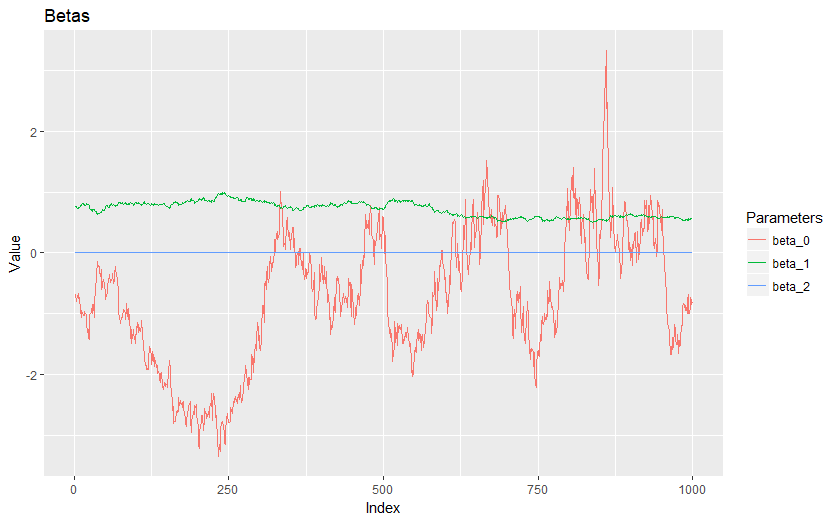
\includegraphics[width=\textwidth]{AnalisisConv/BetaChain}
            \caption{Traza de $\hat{\beta}$}   
            \label{fig:ACBetaChain}
        \end{subfigure}
        \hfill
        \begin{subfigure}[b]{0.45\textwidth}  
            \centering 
            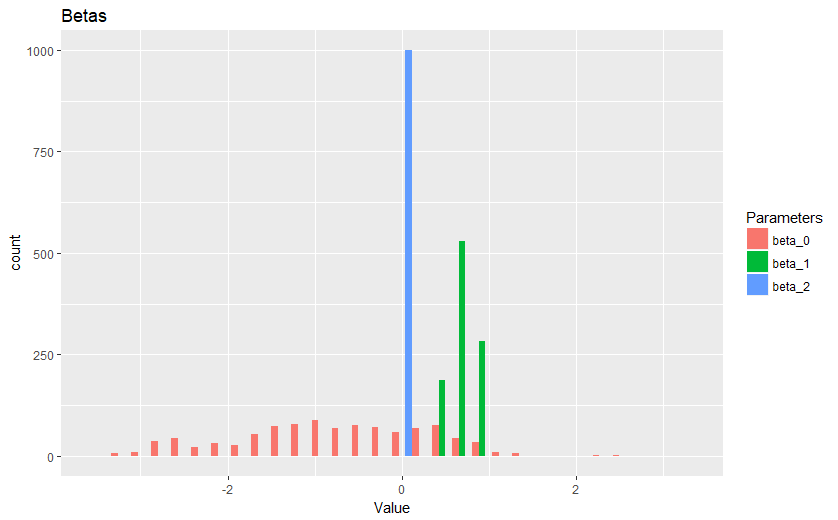
\includegraphics[width=\textwidth]{AnalisisConv/BetaHist}
            \caption{Histograma de $\hat{\beta}$}
            \label{fig:ACBetaHist}
        \end{subfigure}
        \vskip\baselineskip
        \begin{subfigure}[b]{0.45\textwidth}   
            \centering 
            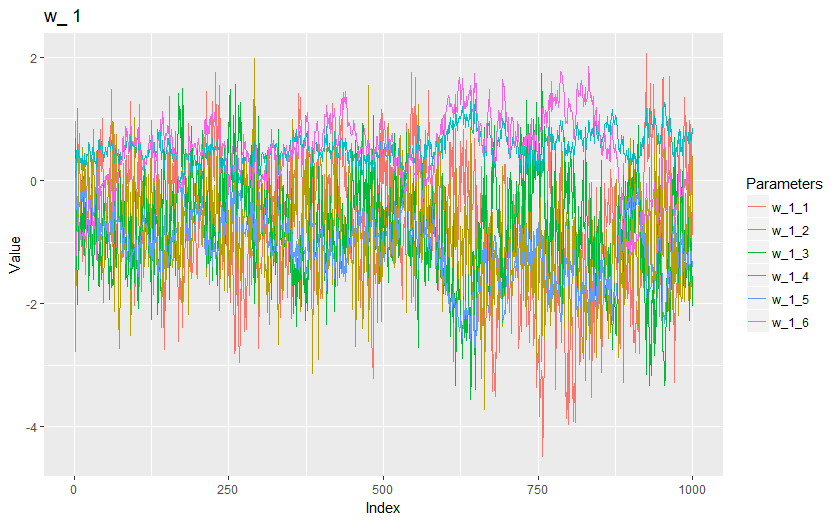
\includegraphics[width=\textwidth]{AnalisisConv/W1Chain}
            \caption{Traza de $\hat{w}_1$}
            \label{fig:ACW1Chain}
        \end{subfigure}
        \quad
        \begin{subfigure}[b]{0.45\textwidth}   
            \centering 
            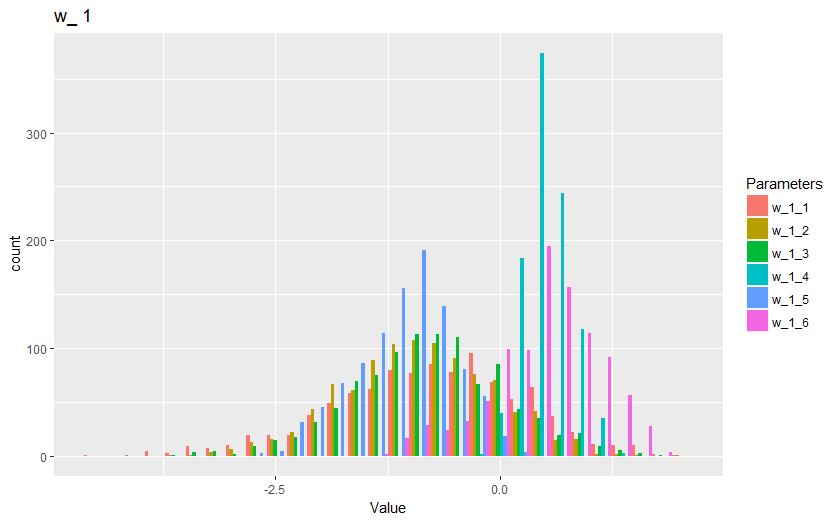
\includegraphics[width=\textwidth]{AnalisisConv/W1Hist}
            \caption{Histograma de $\hat{w}_1$}    
            \label{fig:ACW1Hist}
        \end{subfigure}
                \vskip\baselineskip
        \begin{subfigure}[b]{0.45\textwidth}   
            \centering 
            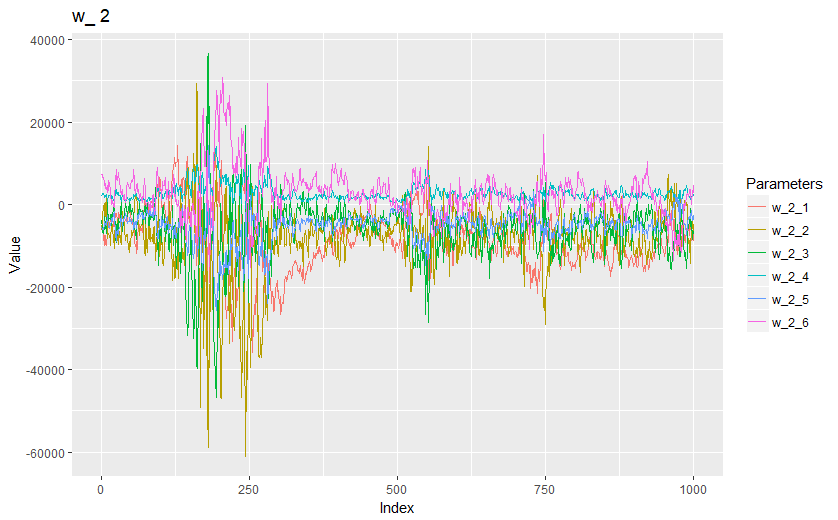
\includegraphics[width=\textwidth]{AnalisisConv/W2Chain}
            \caption{Traza de $\hat{w}_2$}
            \label{fig:ACW2Chain}
        \end{subfigure}
        \quad
        \begin{subfigure}[b]{0.45\textwidth}   
            \centering 
            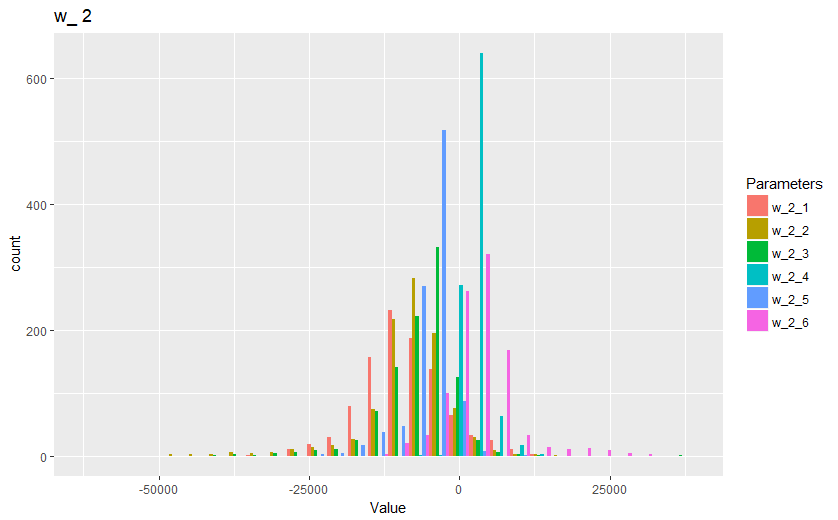
\includegraphics[width=\textwidth]{AnalisisConv/W2Hist}
            \caption{Histograma de $\hat{w}_2$}    
            \label{fig:ACW2Hist}
        \end{subfigure}
        \caption{Trazas e histogramas del ejemplo 6}
        \label{fig:ACGibbs}    
        
  \medskip
  \begin{flushleft}
  \small
Se grafican los últimos 1000 valores de las cadenas del muestreo Gibbs
	\end{flushleft}          
\end{figure}

Algo que queda claro tanto en tablas como en imágenes, es que el parámetro $\hat{\beta}_2$ es idénticamente cero. Aunque pareciera raro, este fenómeno está perfectamente explicado también por la importancia que tiene $\hat{\beta}_1$, al haber explicado los datos únicamente en la primera dimensión con algo de ayuda de $\hat{\beta}_0$, la contribución de $\hat{\beta}_2$ y toda su correspondiente expansión polinómica se puede obviar.\footnote{Este efecto también se debe a la forma que está implementado el algoritmo, los residuales parciales se van capturando de forma ascendente en las dimensiones. Si se hiciera al revés, el parámetro significativo sería $\hat{\beta}_2$ y $\hat{\beta}_1$ sería cero.} Asimismo, dada la falta de ortogonalidad entre las $\hat{\beta}$ y $\hat{\wsn}$, es que los resúmenes numéricos de $\hat{w}_2$ no tienen sentido. Al tener que el parámetro que controla toda la expansión de $j = 2$ es cero, los parámetros $\hat{w}_2$ pueden tomar escalar arbitrarias y fluctuar todo lo quieran sin afectar al modelo. Estas escalas y comportamiento no convergente se ilustra en las imágenes \ref{fig:ACW2Chain} y \ref{fig:ACEMW2Toda}. Sin embargo, al revisar de cerca la figura \ref{fig:ACW2Hist}, se nota que prácticamente todos los parámetros de $\hat{w}_2$ parecieran tener distribuciones normales con media en cero y lo que están haciendo es subir y bajar. La creencia es confirmada por la imagen \ref{fig:ACEMW2Parcial}. Este comportamiento, aunque indeseado, no es atípico. En la práctica, llega a causar problemas de \textit{condicionamiento} de las matrices si las cadenas son muy largas. Por ello, vale la pena \textit{monitoriear} y hacer exploraciones preeliminares para ir descartando parámetros o probando modelos diferentes hasta lograr uno que satisfaga cierto umbral subjetivo del estadista. Para este ejemplo, no tiene mucha relevancia dado que las cadenas convergen rápido, por lo que se toma el segundo parámetro $\hat{\beta}_2$ con motivos ilustrativos.

\begin{figure}[p]
		% Matriz de imágenes de 3x2, los parámetros para abajo, beta, w1, w2 y cada uno chain y hist
        \centering
        \begin{subfigure}[b]{0.45\textwidth}
            \centering
            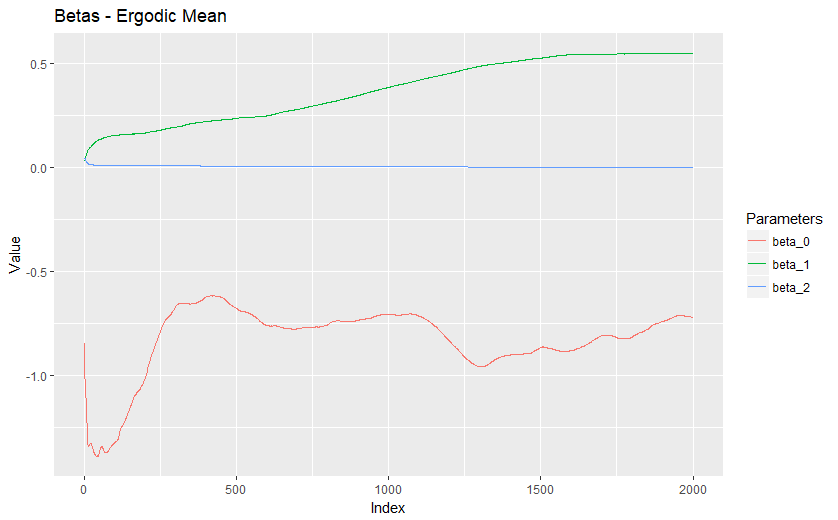
\includegraphics[width=\textwidth]{AnalisisConv/EMBetaToda}
            \caption{Media ergódica para $\hat{\beta}$}   
            \label{fig:ACEMBetaToda}
        \end{subfigure}
        \hfill
        \begin{subfigure}[b]{0.45\textwidth}
            \centering
            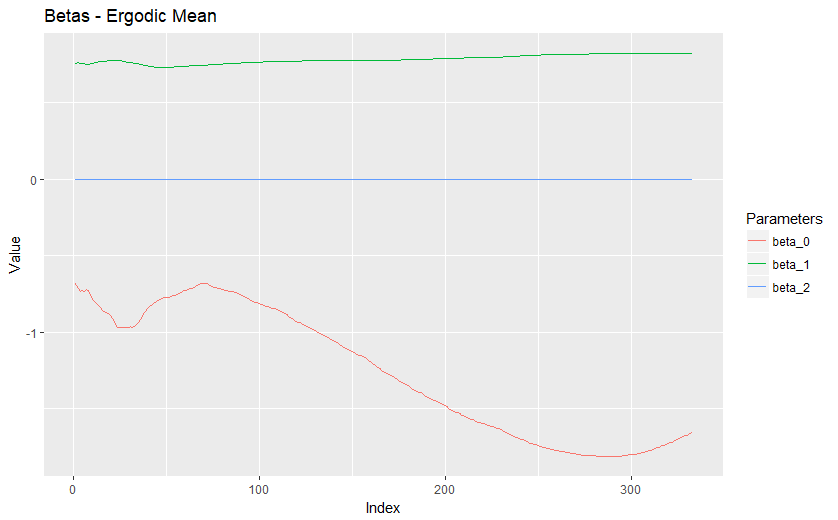
\includegraphics[width=\textwidth]{AnalisisConv/EMBetaParcial}
            \caption{Media ergódica para $\hat{\beta}$ corregida}   
            \label{fig:ACEMBetaParcial}
        \end{subfigure}        
        \vskip\baselineskip        
        \begin{subfigure}[b]{0.45\textwidth}
            \centering
            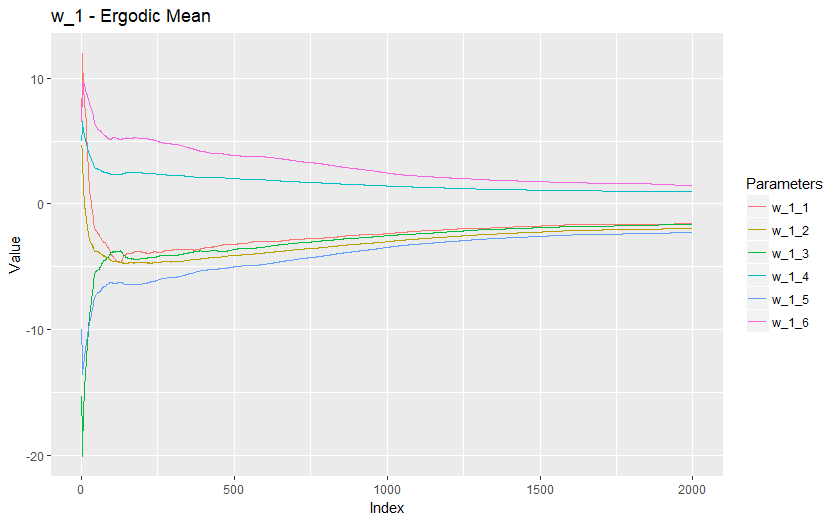
\includegraphics[width=\textwidth]{AnalisisConv/EMW1Toda}
            \caption{Media ergódica para $\hat{w}_1$}   
            \label{fig:ACEMW1Toda}
        \end{subfigure}
        \hfill
        \begin{subfigure}[b]{0.45\textwidth}
            \centering
            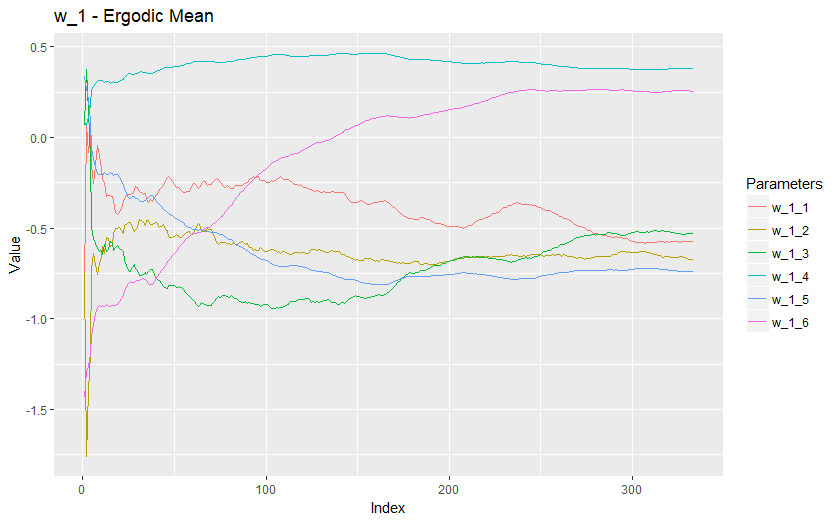
\includegraphics[width=\textwidth]{AnalisisConv/EMW1Parcial}
            \caption{Media ergódica para $\hat{w}_1$ corregida}   
            \label{fig:ACEMW1Parcial}
        \end{subfigure}        
        \vskip\baselineskip
                \begin{subfigure}[b]{0.45\textwidth}
            \centering
            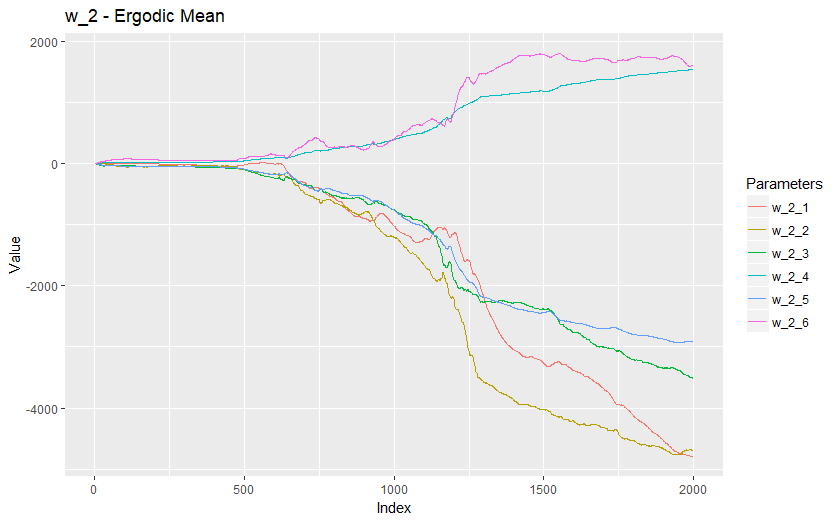
\includegraphics[width=\textwidth]{AnalisisConv/EMW2Toda}
            \caption{Media ergódica para $\hat{w}_2$}   
            \label{fig:ACEMW2Toda}
        \end{subfigure}
        \hfill
        \begin{subfigure}[b]{0.45\textwidth}
            \centering
            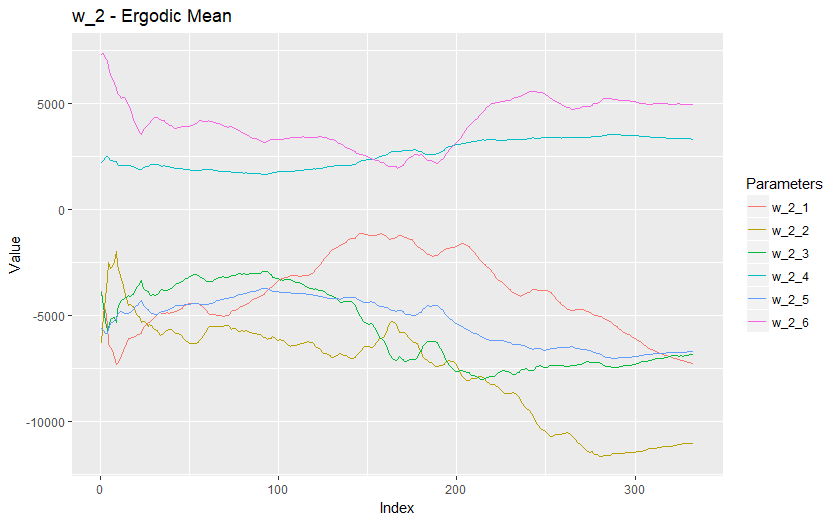
\includegraphics[width=\textwidth]{AnalisisConv/EMW2Parcial}
            \caption{Media ergódica para $\hat{w}_2$ corregida}   
            \label{fig:ACEMW2Parcial}
        \end{subfigure}        
        \caption{Medias ergódicas del ejemplo 6}
        \label{fig:ACEM}
        
          \medskip
  \begin{flushleft}
  \small
En la primera columna, se muestran las medias ergódicas para toda la cadena, es decir, los $\nsim = 2000$ parámetros. En la segunda, se muestran las medias ergódicas para las cadenas corregidas con $k^* = 1000$ y $\kthin = 1000$
	\end{flushleft}          
\end{figure}

Finalmente, se nota la tabla de $\hat{w}_1$. Aunque pareciera se tiene mucha variabilidad en la mayoría de los parámetros, en realidad, se forman cadenas bastante estables que derivan en estimaciones puntuales buenas. Además, la estimación es robusta pues se respeta la normalidad de la distribución posterior derivada de los cálculos bayesianos. Este efecto se ve claramente en la imagen \ref{fig:ACW1Hist}. De esta misma, se nota una clara separación en los parámetros que al final se tomarán negativos y en los positivos, incluso, con procedimientos frecuentistas de pruebas de hipótesis, se podría concluir cuales de ellos pueden ser estadísticamente cero, reduciendo el número de parámetros. Se hace una mención especial a la excelente convergencia de estos parámetros que se nota en las figuras \ref{fig:ACEMW1Toda}
y \ref{fig:ACEMW1Parcial}, al ser realmente importantes para el modelo, controlando la curvatura de la frontera, vale la pena que sean estimados con precisión.

Es interesante notar, que la mayoría de los ejemplos presentados en este trabajo alcanzaron convergencia, pero, esta convergencia no fue tan precisa como gustaría. Sin embargo, los resultados son, sorprendentemente, tan buenos que posiblemente existan relaciones no consideradas que hacen que los parámetros capturen información adicional y hagan excelentes fronteras de predicción. Adicionalmente, estas gráficas son generadas por rutinas del paquete desarrollado para este trabajo, cuya función es automatizar, hasta cierto punto, el análisis de convergencia.

\section{Otros resultados interesantes}
Los ejemplos presentados a continuación, son más expositivos que analíticos, es decir, se enfatizan los resultados y las características fundamentales que los detalles tediosos y técnicos del modelo como se hizo en la sección anterior. Estos ejemplos y bases de datos simuladas, buscan sobre todo, poner a prueba las capacidades no lineales del modelo haciendo predicciones que serían imposibles para un GLM.

% Ej 7 - Normal BiVariada Modificada
\subsubsection*{Una ligera modificación}
Aprovechando la familiaridad de la base de datos anterior, se decidió modificarala para que existieran dos regiones separadas con observaciones del primer grupo. Se tomaron aproximadamente 13 puntos, más allá de $x_1 = 6$ y se cambió su clasificación. Se corre un modelo usando ahora 4 nodos y parábolas continuas resumindo en la Tabla \ref{ej:7}. Los resultados se presentan en la Tabla \ref{tab:Test2Ej7Res} y la Figura \ref{fig:Test2Ej7Plots}.
\begin{table}[h]
$$\paramsmod{3}{4}{1}{9}{2}{350}{1000}{500}{2}$$
\caption{Ejemplo 7, datos normales bivariados modificados}
\label{ej:7}
\end{table}

\begin{table}[h]
\begin{align*}
\resultados{\text{Media posterior}}{98.6}{0.04217}
\qquad\qquad\qquad
\matconf{211}{2}{213}{3}{134}{137}{214}{136}{350}
\end{align*}
\caption{Ejemplo 7, resultados}
\label{tab:Test2Ej7Res}
\end{table}

\begin{figure}[p]
        \centering
        \begin{subfigure}[b]{0.45\textwidth}
            \centering
            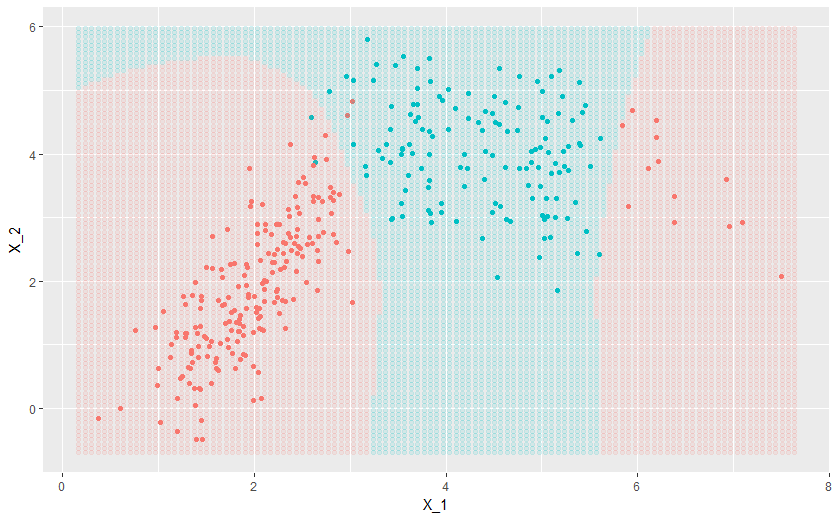
\includegraphics[width=\textwidth]{Tests/Test2/Ej7Frontera}
            \caption{Frontera}   
            \label{fig:Test2Ej7Frontera}
        \end{subfigure}
        \hfill
        \begin{subfigure}[b]{0.45\textwidth}  
            \centering 
            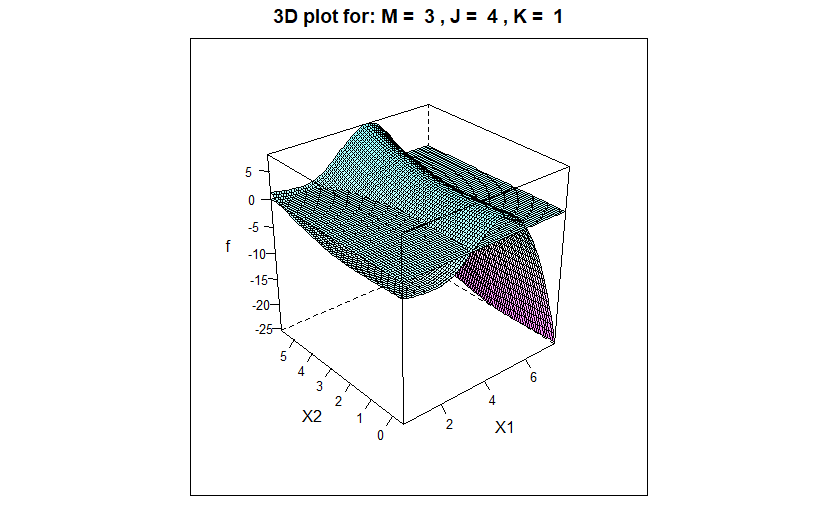
\includegraphics[width=\textwidth]{Tests/Test2/Ej73D}
            \caption{Representación 3D de $\hat{f}$}
            \label{fig:Test2Ej73D}
        \end{subfigure}
        \vskip\baselineskip
        \begin{subfigure}[b]{0.45\textwidth}   
            \centering 
            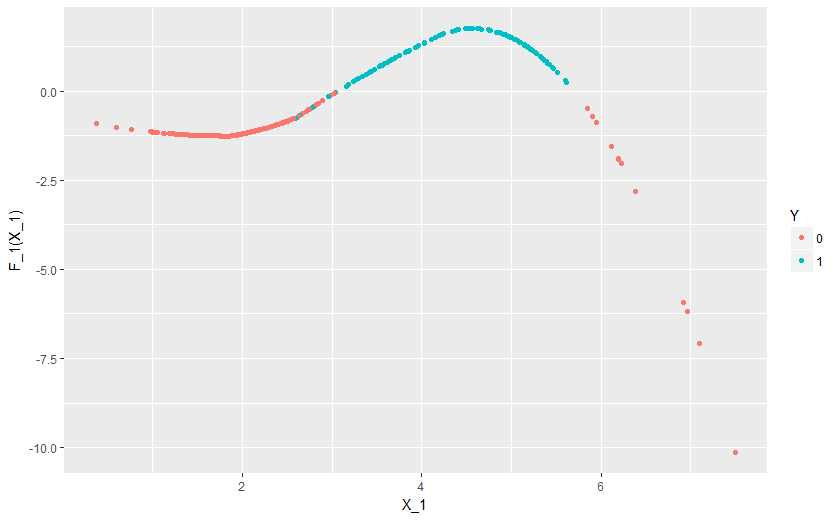
\includegraphics[width=\textwidth]{Tests/Test2/Ej7F1}
            \caption{$\hat{f}_1(x_1)$}
            \label{fig:Test2Ej7F1}
        \end{subfigure}
        \quad
        \begin{subfigure}[b]{0.45\textwidth}   
            \centering 
            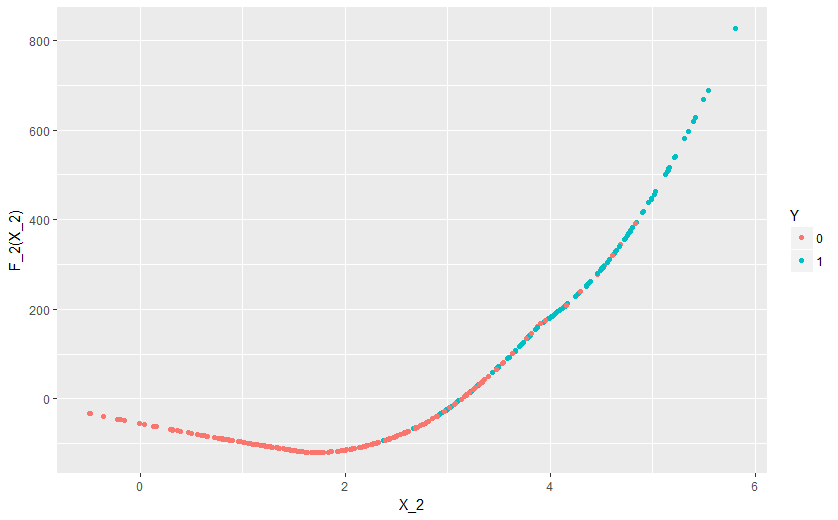
\includegraphics[width=\textwidth]{Tests/Test2/Ej7F2}
            \caption{$\hat{f}_2(x_2)$}    
            \label{fig:Test2Ej7F2}
        \end{subfigure}
        \caption{Ejemplo 7 con $M = 3$, $J = 4$, $K = 1$}
        \label{fig:Test2Ej7Plots}
\end{figure}

Este ejemplo es interesante pues, como se ve en la imágen \ref{fig:Test2Ej73D}, la \textit{sabana} que antes era creciente a medida que $x_1$ crecía, ahora se vuelve a curvar, volviéndose negativa otra vez y clasificando bien la segunda sección roja. Una vez más, se tienen esos pocos puntos que no quedan bien clasificados, incluyendo uno nuevo cerca de las coordenadas cartesianas $(5.8, 2.3)$. Para estos datos, se debe usar un nodo adicional cerca de la segunda región, ya que la curvatura, deriva de él. El parámetro $K$ en este ejemplo no es muy relevante como se ve en la imagen \ref{fig:Test2Ej7F1}, nuevamente porque $\hat{f}_1(x_1)$ pareciera ser suficientemente suave sin tener que restringir el modelo. Finalmente, se enfatiza que vuelve a suceder lo mismo que pasó con el ejemplo 6, donde la información se podía resumir únicamente con las primeras dos dimensiones. 

% Ej 9 y 10 - Parabola y Circular Data
\subsubsection{Regiones curvas}
Como siguientes dos ejemplos, se buscó estresar la interacción entre las dimensiones buscando regiones más complejas. En particular, se buscó replicar algo similar a la imagen del capítulo introductorio \ref{fig:DiagramaIntro} de la página \pageref{fig:DiagramaIntro}. Para el ejemplo 8, se generaron datos con coordenadas polares para ángulos con rango entre $(-1,1)$ y tomando diferentes radios para cada grupo. Posteriormente, se les sumó ruido blanco a los puntos para que existiera una región de confusión. Dadas las características curvas de los datos, piensa que usar parábolas continuas es una buena opción para modelarlos. El modelo final termina con los parámetros presentados en la Tabla \ref{ej:8}. Los resultados e imágenes se presentan en la Tabla \ref{tab:Test3Ej8Res} y la Figura \ref{fig:Test3Ej8Plots} respectivamente.

\begin{table}[h]
$$\paramsmod{3}{4}{1}{9}{2}{400}{1000}{500}{1}$$
\caption{Ejemplo 8, datos parabólicos anidados}
\label{ej:8}
\end{table}

\begin{table}[h]
\begin{align*}
\resultados{\text{Media posterior}}{98.8}{0.04217}
\qquad\qquad\qquad
\matconf{196}{4}{200}{1}{199}{200}{197}{203}{400}
\end{align*}
\caption{Ejemplo 8, resultados}
\label{tab:Test3Ej8Res}
\end{table}

\begin{figure}[p]
        \centering
        \begin{subfigure}[b]{0.45\textwidth}
            \centering
            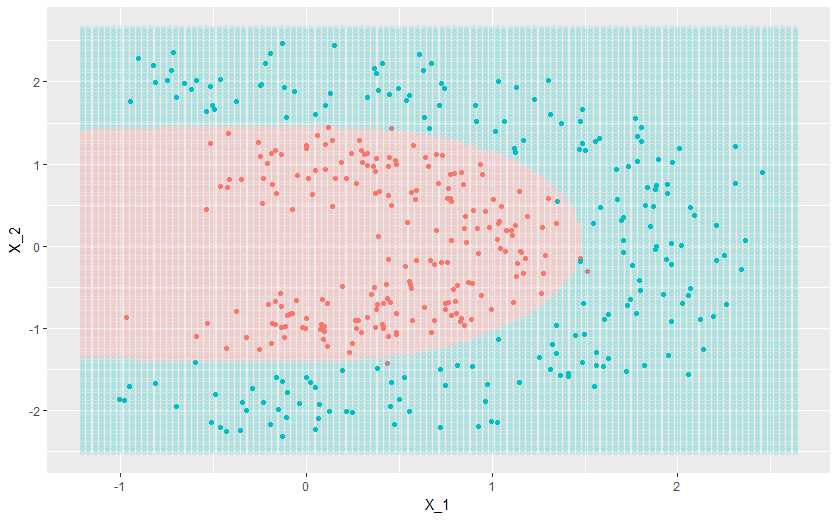
\includegraphics[width=\textwidth]{Tests/Test3/Ej8Frontera}
            \caption{Frontera}   
            \label{fig:Test3Ej8Frontera}
        \end{subfigure}
        \hfill
        \begin{subfigure}[b]{0.45\textwidth}  
            \centering 
            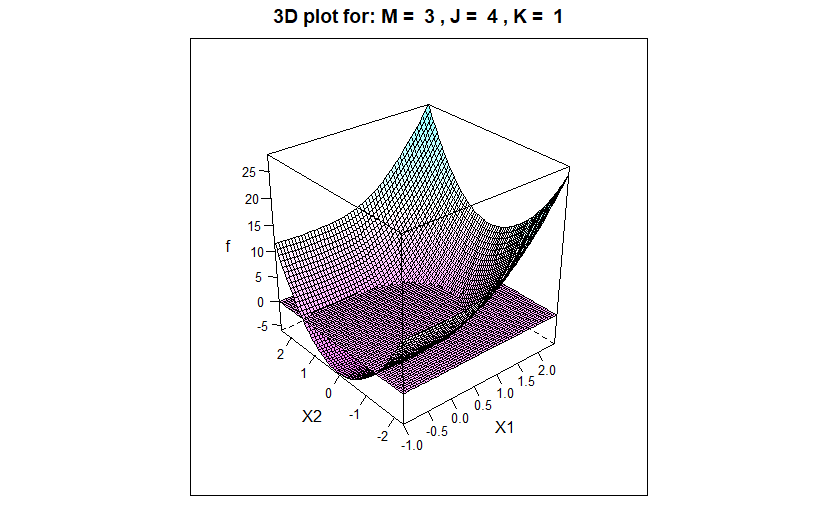
\includegraphics[width=\textwidth]{Tests/Test3/Ej83D}
            \caption{Representación 3D de $\hat{f}$}
            \label{fig:Test3Ej83D}
        \end{subfigure}
        \vskip\baselineskip
        \begin{subfigure}[b]{0.45\textwidth}   
            \centering 
            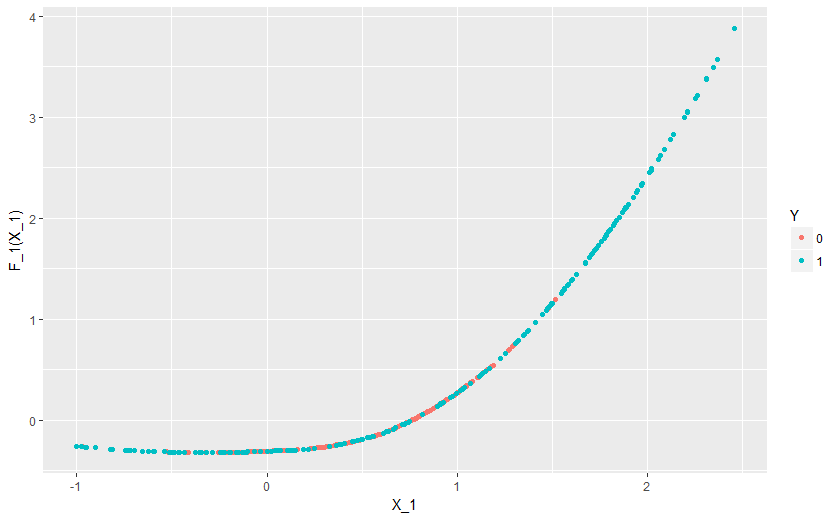
\includegraphics[width=\textwidth]{Tests/Test3/Ej8F1}
            \caption{$\hat{f}_1(x_1)$}
            \label{fig:Test3Ej8F1}
        \end{subfigure}
        \quad
        \begin{subfigure}[b]{0.45\textwidth}   
            \centering 
            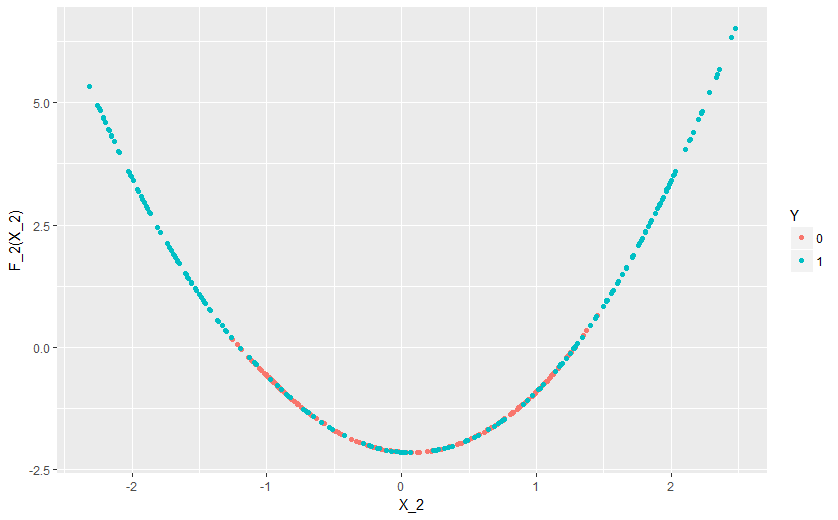
\includegraphics[width=\textwidth]{Tests/Test3/Ej8F2}
            \caption{$\hat{f}_2(x_2)$}    
            \label{fig:Test3Ej8F2}
        \end{subfigure}
        \caption{Ejemplo 8 con $M = 3$, $J = 4$, $K = 1$}
        \label{fig:Test3Ej8Plots}
\end{figure}
Este es un modelo particularmente interesante de forma gráfica. Se ve claramente que la segunda dimensión \ref{fig:Test3Ej8F2} captura la parte parabólica y la primera \ref{fig:Test3Ej8F2}, la región donde se confunden los grupos pero posteriormente hay certidumbre. A diferencia de los modelos presentados hasta ahora, todos los parámetros $\beta$ son altamente significantes, pues sin su interacción, claramente no se habría detectado el patrón. Sin embargo, estos datos siguen teniendo una clara separación por lo que el modelo sigue logrando detectar la frontera de forma correcta y tener precisión.

Continuando con las regiones no lineales, se obtuvo una base de datos pequeña del curso online de Machine Learning de \citet{andrew2018ml}.\footnote{Este curso, se ofrece de forma gratuita en la página de \href{https://www.coursera.org/learn/machine-learning}{Coursera}} Esta base de datos se usa para entrenar modelos saturados logit con regularización, logrando predecir fronteras circulares con modelos lineales. Se decidió, probarlo también con el modelo a ver si se obtenían resultados comparables. Efectivamente se logró y con un menor número de parámetros por entrenar. El modelo, una vez más, fue ajustado con parábolas continuas las cuales resultaron ser excelentes herramientas. Se tiene el ejemplo 9 resumido en la Tabla \ref{ej:9}, con resultados e imágenes en la Tabla \ref{tab:Test4Ej9Res} y Figura \ref{fig:Test4Ej9Plots} respectivamente. 

\begin{table}[h]
$$\paramsmod{3}{4}{2}{6}{2}{118}{1000}{500}{1}$$
\caption{Ejemplo 9, datos circulares}
\label{ej:9}
\end{table}

\begin{table}[h]
\begin{align*}
\resultados{\text{Media posterior}}{78.8}{0.4532}
\qquad\qquad\qquad
\matconf{48}{12}{60}{13}{45}{58}{61}{44}{118}
\end{align*}
\caption{Ejemplo 9, resultados}
\label{tab:Test4Ej9Res}
\end{table}

\begin{figure}[p]
        \centering
        \begin{subfigure}[b]{0.45\textwidth}
            \centering
            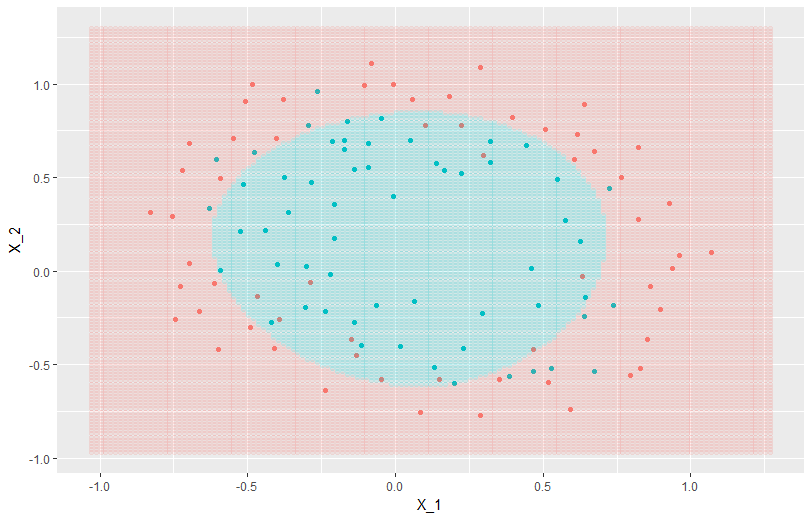
\includegraphics[width=\textwidth]{Tests/Test4/Ej9Frontera}
            \caption{Frontera}   
            \label{fig:Test4Ej9Frontera}
        \end{subfigure}
        \hfill
        \begin{subfigure}[b]{0.45\textwidth}  
            \centering 
            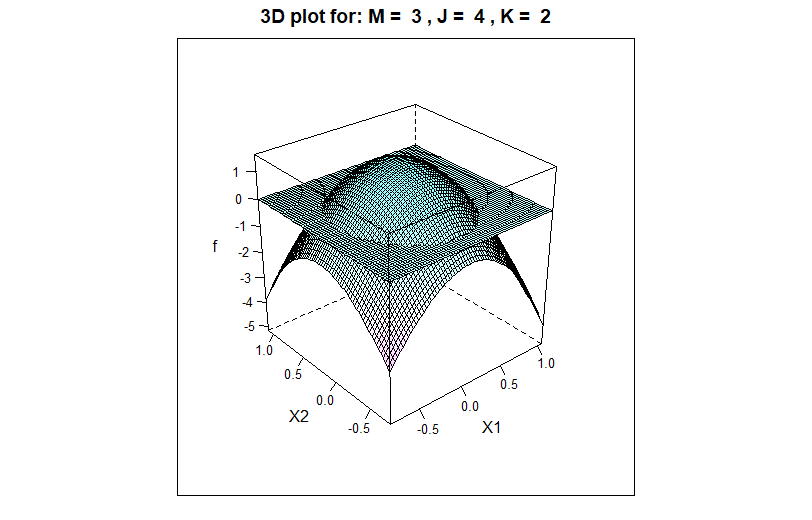
\includegraphics[width=\textwidth]{Tests/Test4/Ej93D}
            \caption{Representación 3D de $\hat{f}$}
            \label{fig:Test4Ej93D}
        \end{subfigure}
        \vskip\baselineskip
        \begin{subfigure}[b]{0.45\textwidth}   
            \centering 
            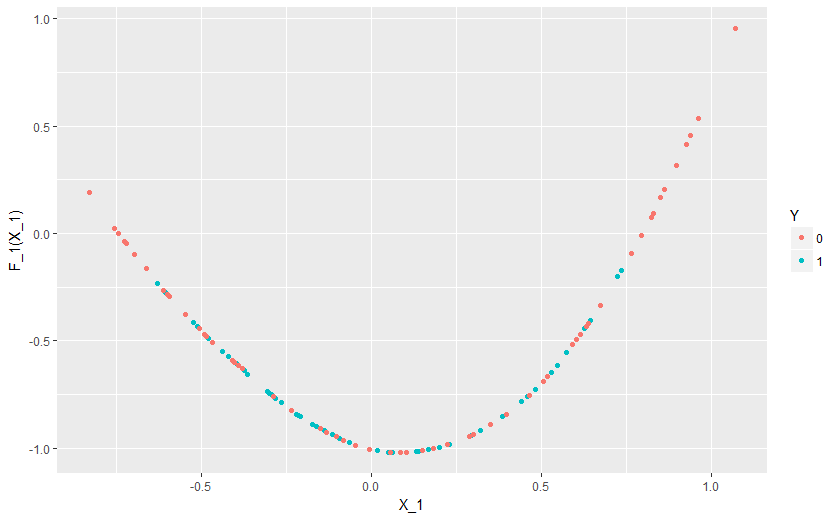
\includegraphics[width=\textwidth]{Tests/Test4/Ej9F1}
            \caption{$\hat{f}_1(x_1)$}
            \label{fig:Test4Ej9F1}
        \end{subfigure}
        \quad
        \begin{subfigure}[b]{0.45\textwidth}   
            \centering 
            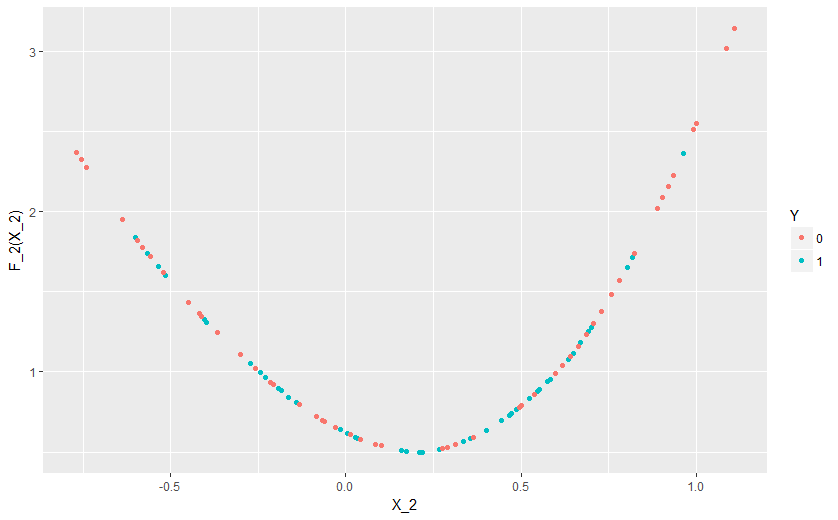
\includegraphics[width=\textwidth]{Tests/Test4/Ej9F2}
            \caption{$\hat{f}_2(x_2)$}    
            \label{fig:Test4Ej9F2}
        \end{subfigure}
        \caption{Ejemplo 9 con $M = 3$, $J = 4$, $K = 2$}
        \label{fig:Test4Ej9Plots}
\end{figure}

Todo el poder del modelo, recae en esta forma de romper la linealidad y poder estimar regiones irregularmente curvas, incluso con muy pocas observaciones. El modelo tiene un total de $15$ parámetros,\footnote{3 en beta $\beta$ más $2\times6$ de los vectores $w_j$} cuando en el curso, se entrenaba con 28 parámetros.\footnote{Cabe mencionar que, dada la regularización, muchos de estos términos ser desvanecían.} La forma en la que interactún los nodos, combinando las dos parábolas que se forman en \ref{fig:Test4Ej9F1} y \ref{fig:Test4Ej9F1} es muy interesante, pues, aunque se tienen 3 nodos, lo optimo para estas figuras es formar dos parábolas continuas y suaves al aumentar $K$. 

\subsubsection*{Ultimo ejemplo con datos simulados - limitaciones del modelo}
Para finalizar con las  bases de datos simulados, el modelo se llevó al límite de sus capacidades sobre un patrón de puntos, intuitivo al ojo humano, pero realmente difícil de identificar por un algoritmo.\footnote{O al menos el presentado en este trabajo} Los datos tratan de simular un \textit{yin-yang} que se puede ver en la Figura \ref{fig:YYDatos}. La simple simulación de la base de datos representó un reto donde se conjuntaron varias áreas de la matemática aplicada. En el software \verb|GeoGebra|, se generó el diagrama presentado en la Figura \ref{fig:YYGG} que consiste de las siguientes desigualdades cartesianas:
\begin{align*}
	x^2 + y^2 &< 16, \\
	(x+2)^2 + (y-1.5)^2 &< 0.49, \\
	(x-1.5)^2 + (y+2)^2 &< 0.49, \\[4pt]
	x &< \dfrac{y}{(1+y^2).}
\end{align*}

\begin{figure}[h]
        \centering
        \begin{subfigure}[b]{0.45\textwidth}
            \centering
            \includegraphics[width=\textwidth]{Tests/Test5/YYDatos}
            \caption{Datos simulados representando un yin-yang}   
            \label{fig:YYDatos}
        \end{subfigure}
        \hfill
        \begin{subfigure}[b]{0.45\textwidth}  
            \centering 
            \includegraphics[width=\textwidth]{Tests/Test5/YYGG}
            \caption{Salida del software donde se construyeron las ecuaciones para generar los datos.}
            \label{fig:YYGG}
        \end{subfigure}
        \caption{Patrón yin-yang}
        \label{fig:YYInitialPlots}
\end{figure}
Una vez \textit{dibujadas} las ecuaciones, se generaron dos bases de datos de aproximadamente $n \approx 1500$ observaciones. La primera, con distribución uniforme dentro del círculo,\footnote{Usando coordenadas polares} y otra usando una distribución normal bivariada simétrica ($\rho = 0$) pero con desviación estándar $\sigma = 2.5$ para abarcar todo el circulo. A todos estos puntos se les asignó la categoría 0, posteriormente, se asignó la categoría 1 a los puntos que cayeran en las regiones deseadas. Al final, se le añadió algo de ruido normal a cada punto para darle aleatoriedad a la base de datos pero manteniendo el patrón terminando así la simulación.

El modelo se corrió, con muchas esperanzas, un sinfín de veces, tratando de calibrar los parámetros y captar exactamente el patrón. Sin embargo y aunque el modelo casi siempre lograba una precisión de cerca de $85\%$, no se lograron los resultados esperados. De cualquier forma, el modelo y el algoritmo, claramente están haciendo su mejor trabajo y los parámetros convergen. En la Figura \ref{fig:YY} se pueden ver las fronteras de algunos de los mejores modelos.

\begin{figure}[p]
        \centering
        \begin{subfigure}[b]{0.45\textwidth}
            \centering
            \includegraphics[width=\textwidth]{Tests/Test5/YY1}
            \caption{Datos uniformes sin ruido, buen ajuste}
			\label{fig:YY1}
        \end{subfigure}
        \hfill
        \begin{subfigure}[b]{0.45\textwidth}  
            \centering 
            \includegraphics[width=\textwidth]{Tests/Test5/YY2}
            \caption{Datos uniformes con ruido, mejor modelo}
			\label{fig:YY2}
        \end{subfigure}
        \vskip\baselineskip
        \begin{subfigure}[b]{0.45\textwidth}
            \centering
            \includegraphics[width=\textwidth]{Tests/Test5/YY3}
			\caption{Datos normales con ruido}
			\label{fig:YY3}
        \end{subfigure}
        \hfill
        \begin{subfigure}[b]{0.45\textwidth}  
            \centering 
            \includegraphics[width=\textwidth]{Tests/Test5/YY3D}
			\caption{Gráfico 3D para uno de los modelos}
			\label{fig:YY3D}
        \end{subfigure}
    	\caption{Fronteras de varios modelos para datos yin-yang}
        \label{fig:YY}
\end{figure}
Para las dos primeras imágenes \ref{fig:YY1} y \ref{fig:YY2}, se usa la base de datos uniformes, la primera sin ruido y la siguiente con. El agregarle ruido, hace que los datos no sean tan uniformes en el espacio y que ciertas características se vuelvan más prominentes que otras. Es por ello, que en la segunda imagen, se logró detectar la zona roja de la izquierda, a costa de perder algunas observaciones azules en el \textit{puente} que se forma para llegar a ella. Sin embargo, en la primera imagen, el modelo no sólo detectó relativamente bien la curva de en medio, sino que detecta de forma aislada, el circulo azul de la esquina inferior derecha. En la tercera imagen \ref{fig:YY3}, se usan los datos normales con ruido de donde se ve claramente que el modelo detecta que existen regiones que debería de estar estimando dentro de las categorías opuestas. Finalmente \ref{fig:YY3D}, muestra una, de las muchas representaciones 3D que se hicieron al tratar de ajustar esta base de datos. 

Precisamente en esta última imagen se esconde el porqué no se logró hacer la estimación correcta: la dependencia implícita entre los nodos. Estos nodos, en realidad están dividiendo el espacio bi-dimensional en una cuadrícula donde las interacciones son difíciles de discernir. Conforme aumenta el número de nodos, más complejo se vuelve el modelo. Es por ello, que los picos y valles se repiten en un patrón uniforme. Asimismo, dada la naturaleza global de los polinomios y esta interacción, el modelo tiene esta estructura decreciente siempre, derivando que los picos y los valles nunca alcancen las regiones extremas en polos opuestos. De igual forma, la uniformidad y simetría impar, inherente a esta base de datos, llevó a que la estimación de los parámetros fuera óptima dentro de las capacidades del modelo. Otra desventaja de esta base, es que estos modelos se tuvieron que correr con un número grande de nodos $J \approx 20$, derivando en un número de parámetros aún más alto $\N \approx 50$. Sin embargo, el tiempo de estimación para cadenas de más de 4000 observaciones y alrededor de 100 parámetros, nunca excedió el minuto. 

\section{Prueba con datos médicos reales}
Aunque interesantes, hasta ahora, todos los resultados de este trabajo han sido sobre bases de datos simuladas sin trascendencia alguna. Claramente forman imágenes atractivas por construcción, pero no se está prediciendo nada ni formando modelos aplicables en la vida real. Por lo tanto, y para hacer una última prueba de el modelo, se presenta una base de datos de cáncer de mama de la Univeridad de Wisconsin. Esta base de datos, es citada en varios trabajos de los años noventa, donde se tratan de hacer clasificaciones binarias usando una serie de procedimientos más robustos que los tradicionales GLM \autocite{mangasarian1990pattern}, \autocite{bennett1992robust}.

De manera general y sin entrar en la parte médica de las variables como tal, se presenta un análisis exploratorio preliminar que se lleva a cabo para seleccionar las que se consideren relevantes. La base de datos cuenta con $n = 699$ observaciones de las cuales el $34.5\%$ representan pacientes infectados con tumores malignos representados por el color rojo. Se cuenta con diez variables (dimensiones) médicas sobre las características de los tumores como lo son: el tamaño, la uniformidad de la pared celular, etcétera. En la Figura \ref{fig:BCExp}, se muestran los gráficos de puntos \textit{pareados} para todas las posibles combinaciones, además de información adicional.
\begin{figure}[h]
	\centering
	\includegraphics[width=.9\textwidth]{Tests/Test6/BCExp}
	\caption{Análisis exploratorio para selección de variables}
	\label{fig:BCExp}
\end{figure}
Este proceso, se lleva a cabo para tratar de seleccionar las variables relevantes y/o, discernir alguna región que se pueda separar por proyectores no lineales. Se hace notar que las variables, están codificadas en una escala a 10 puntos, por lo tanto, la representación gráfica de los datos se ve más como una cuadrícula que como un espacio real de variables. Se seleccionan las variables \textit{clump, size} y \textit{chromatin}\footnote{Estas variables corresponden a el espesor de los tumores, su tamaño y la textura de la cromatina en las células respectivamente} debido a que pareciera ser las que mejor separan el espacio. En la Figura \ref{fig:BCJP} se presentan dos gráficos de puntos con algo de ruido para hacer notar que las regiones son un poco más complejas de lo que podría parecer a simple vista, además de que se tienen puntos idénticos con clasificaciones contrarias. Sin embargo, si se detecta cierto patrón en los datos.
\begin{figure}[h]
        \centering
        \begin{subfigure}[b]{0.45\textwidth}
            \centering
            \includegraphics[width=\textwidth]{Tests/Test6/BCJP1}
            \caption{Variables \textit{clump} y \textit{chromatin}}
			\label{fig:BCJP1}
        \end{subfigure}
        \hfill
        \begin{subfigure}[b]{0.45\textwidth}  
            \centering 
            \includegraphics[width=\textwidth]{Tests/Test6/BCJP1}
            \caption{Variables \textit{clump} y \textit{size} con algo de ruido para separar las observaciones.}
			\label{fig:BCJP2}
        \end{subfigure}
		\caption{Gráficos con  ruido para separar las observaciones}
		\label{fig:BCJP}
\end{figure}

Para poder hablar de \textit{predicción} como tal, tiene que existir una base de datos contra la cual probar las estimaciones del modelo. Por lo tanto, la base original se decide partir en dos, un conjunto de entrenamiento con el $60\%$ de las observaciones ($n=274$) y un conjunto de prueba, con las observaciones restantes sobre las que se evaluará el modelo.\footnote{La diferencia de 16 observaciones entre la suma de entrenamiento y prueba, contra las 699 originales, se debe a que estas estaban incompletas y por lo tanto se descartan.} El modelo final, se resume en la Tabla \ref{ej:BC}, y consta de parábolas continuas con cuatro nodos. Como de costumbre, los resultados numéricos se presentan en la Tabla \ref{tab:BCRes}.
\begin{table}[h]
$$\paramsmod{3}{5}{1}{11}{3}{409}{4000}{3000}{0}$$
\caption{Prueba con datos médicos reales}
\label{ej:BC}
\end{table}

\begin{table}
\begin{align*}
\resultados{\text{Media posterior}}{96}{0.2199}
\qquad\qquad\qquad
\matconf{170}{8}{178}{3}{93}{96}{173}{101}{274}
\end{align*}
\caption{Datos médicos, resultados}
\label{tab:BCRes}
\end{table}

Estos resultados son excelentes pues, incluso haciendo una predicción \textit{fuera de muestra} se logra una precisión del $96\%$, significando, que inclusive en $d=3$ el modelo logra hacer una buena separación. Sin embargo, derivado también de lo mismo, es que no se pueden hacer visualizaciones como en los ejemplos anteriores. La convergencia es clara aunque, si se revisan los resultados numéricos, las escalas son relativamente arbitrarias. El algoritmo, aunque bueno en general, sufre de un problema de estabilidad numérica. Al aumentar el número de parámetros, sobre todo a través de $d$, las cadenas empiezan a divergir mucho y muy rápido, haciendo que la estimación de los parámetros sea errónea. Por lo pronto y para $d\leq4$, el algoritmo funciona bien para cadenas cortas y, aunque pueda ser inestable a la larga, da resultados predictivos muy buenos. De igual manera, para esta base de datos, la codificación de las variables usando una escala de 10 puntos, no es óptima para el modelo pues los nodos se asumen reales. 
\end{document}